\chapter{HASIL DAN PEMBAHASAN}

\section{\textit{Preprocessing}}
Data yang digunakan pada penelitian ini yaitu Dataset ISIC 2019 dengan 1600 data citra kanker kulit yang terdiri dari 8 kelas dan memiliki ukuran $1024\times 1024$ piksel. Mempertimbangkan ukuran data masukan metode YOLOv7 sebesar $640\times 640$, penelitian ini melakukan \textit{resize} untuk proses \textit{preprocessing} menggunakan metode \textit{Bilinear Interpolation} seperti pada Persamaan \ref{eq:resize}. Setelah melakukan proses \textit{resize}, penelitian ini melakukan \textit{annotation} untuk proses \textit{preprocessing} yang berguna untuk proses pelatihan model YOLOv7.
    \subsection{\textit{Resize}}
    Pada penelitian ini, tahap awal untuk melakukan klasifikasi jenis kanker kulit menggunakan metode YOLO adalah tahap \textit{preprocessing}. Seiring berkembangnya waktu, metode YOLO semakin meningkatkan kompleksitasnya sehingga sangat diperlukan optimasi di dibidang waktu komputasi. Salah satu untuk menguranginya adalah melakukan \textit{resize} sesuai ukuran masukan YOLO. Penelitian ini menggunakan YOLOv7 sebagai metode klasifikasi jenis kanker kulit dan YOLOv7 menggunakan ukuran data masukan $640\times 640$ piksel. Dataset ISIC 2019 yang awalnya berukuran $1024\times 1024$ piksel dilakukan \textit{resize} ke dalam ukuran $640\times 640$ piksel menggunakan rumus pada Persamaan \ref{eq:resize}. Perhitungan setiap piksel untuk mengubah ukuran citra dari ukuran $1024\times 1024$ ke dalam ukuran $640\times 640$ seperti di bawah ini.

    \begin{align*}
        (0,0) \Rightarrow Z     &=  &&A (1-w_x) (1-w_y) + B w_x (1-w_y) + C (1-w_x) w_y + \\
                                &   &&D w_x w_y\\
                                &=  &&214\times (1-0)\times (1-0) + 214\times 0\times (1-0) + 214 \times \\
                                &   &&(1-0)\times 0 + 214\times 0\times 0\\
                                &=  &&214\\
        (0,1) \Rightarrow Z     &=  &&A (1-w_x) (1-w_y) + B w_x (1-w_y) + C (1-w_x) w_y + \\
                                &   &&D w_x w_y\\
                                &=  &&228\times (1-0.7)\times (1-0) + 227\times 0.7\times (1-0) + 228 \times \\
                                &   &&(1-0.7)\times 0 + 227\times 0.7\times 0\\
                                &=  &&227\\
        \vdots\\
        (639,639) \Rightarrow Z &=  &&A (1-w_x) (1-w_y) + B w_x (1-w_y) + C (1-w_x) w_y + \\
                                &   &&D w_x w_y\\
                                &=  &&212\times (1-0.3)\times (1-0) + 211\times 0.3\times (1-0) + 212 \times \\
                                &   &&(1-0.3)\times 0 + 211\times 0.3\times 0\\
                                &=  &&212\\
    \end{align*}
    
    Dimana $Z$ merupakan nilai piksel yang baru, $A$, $B$, $C$, $D$ merupakan nilai piksel pada titik-titik terdekat, $w_x$ merupakan bobot koordinat $x$, dan $w_y$ merupakan bobot koordinat $y$. Perhitungan nilai piksel dilakukan dari titik koordinat $(0, 0)$ hingga titik koordinat $(639, 639)$ seperti perhitungan di atas. Berdasarkan perhitungan di atas, hasil \textit{resize} pada dataset ISIC 2019 seperti terlihat pada Gambar \ref{fig:d-resized}.

    \begin{figure}[H]
        \centering
        \begin{tabular}{cc}
            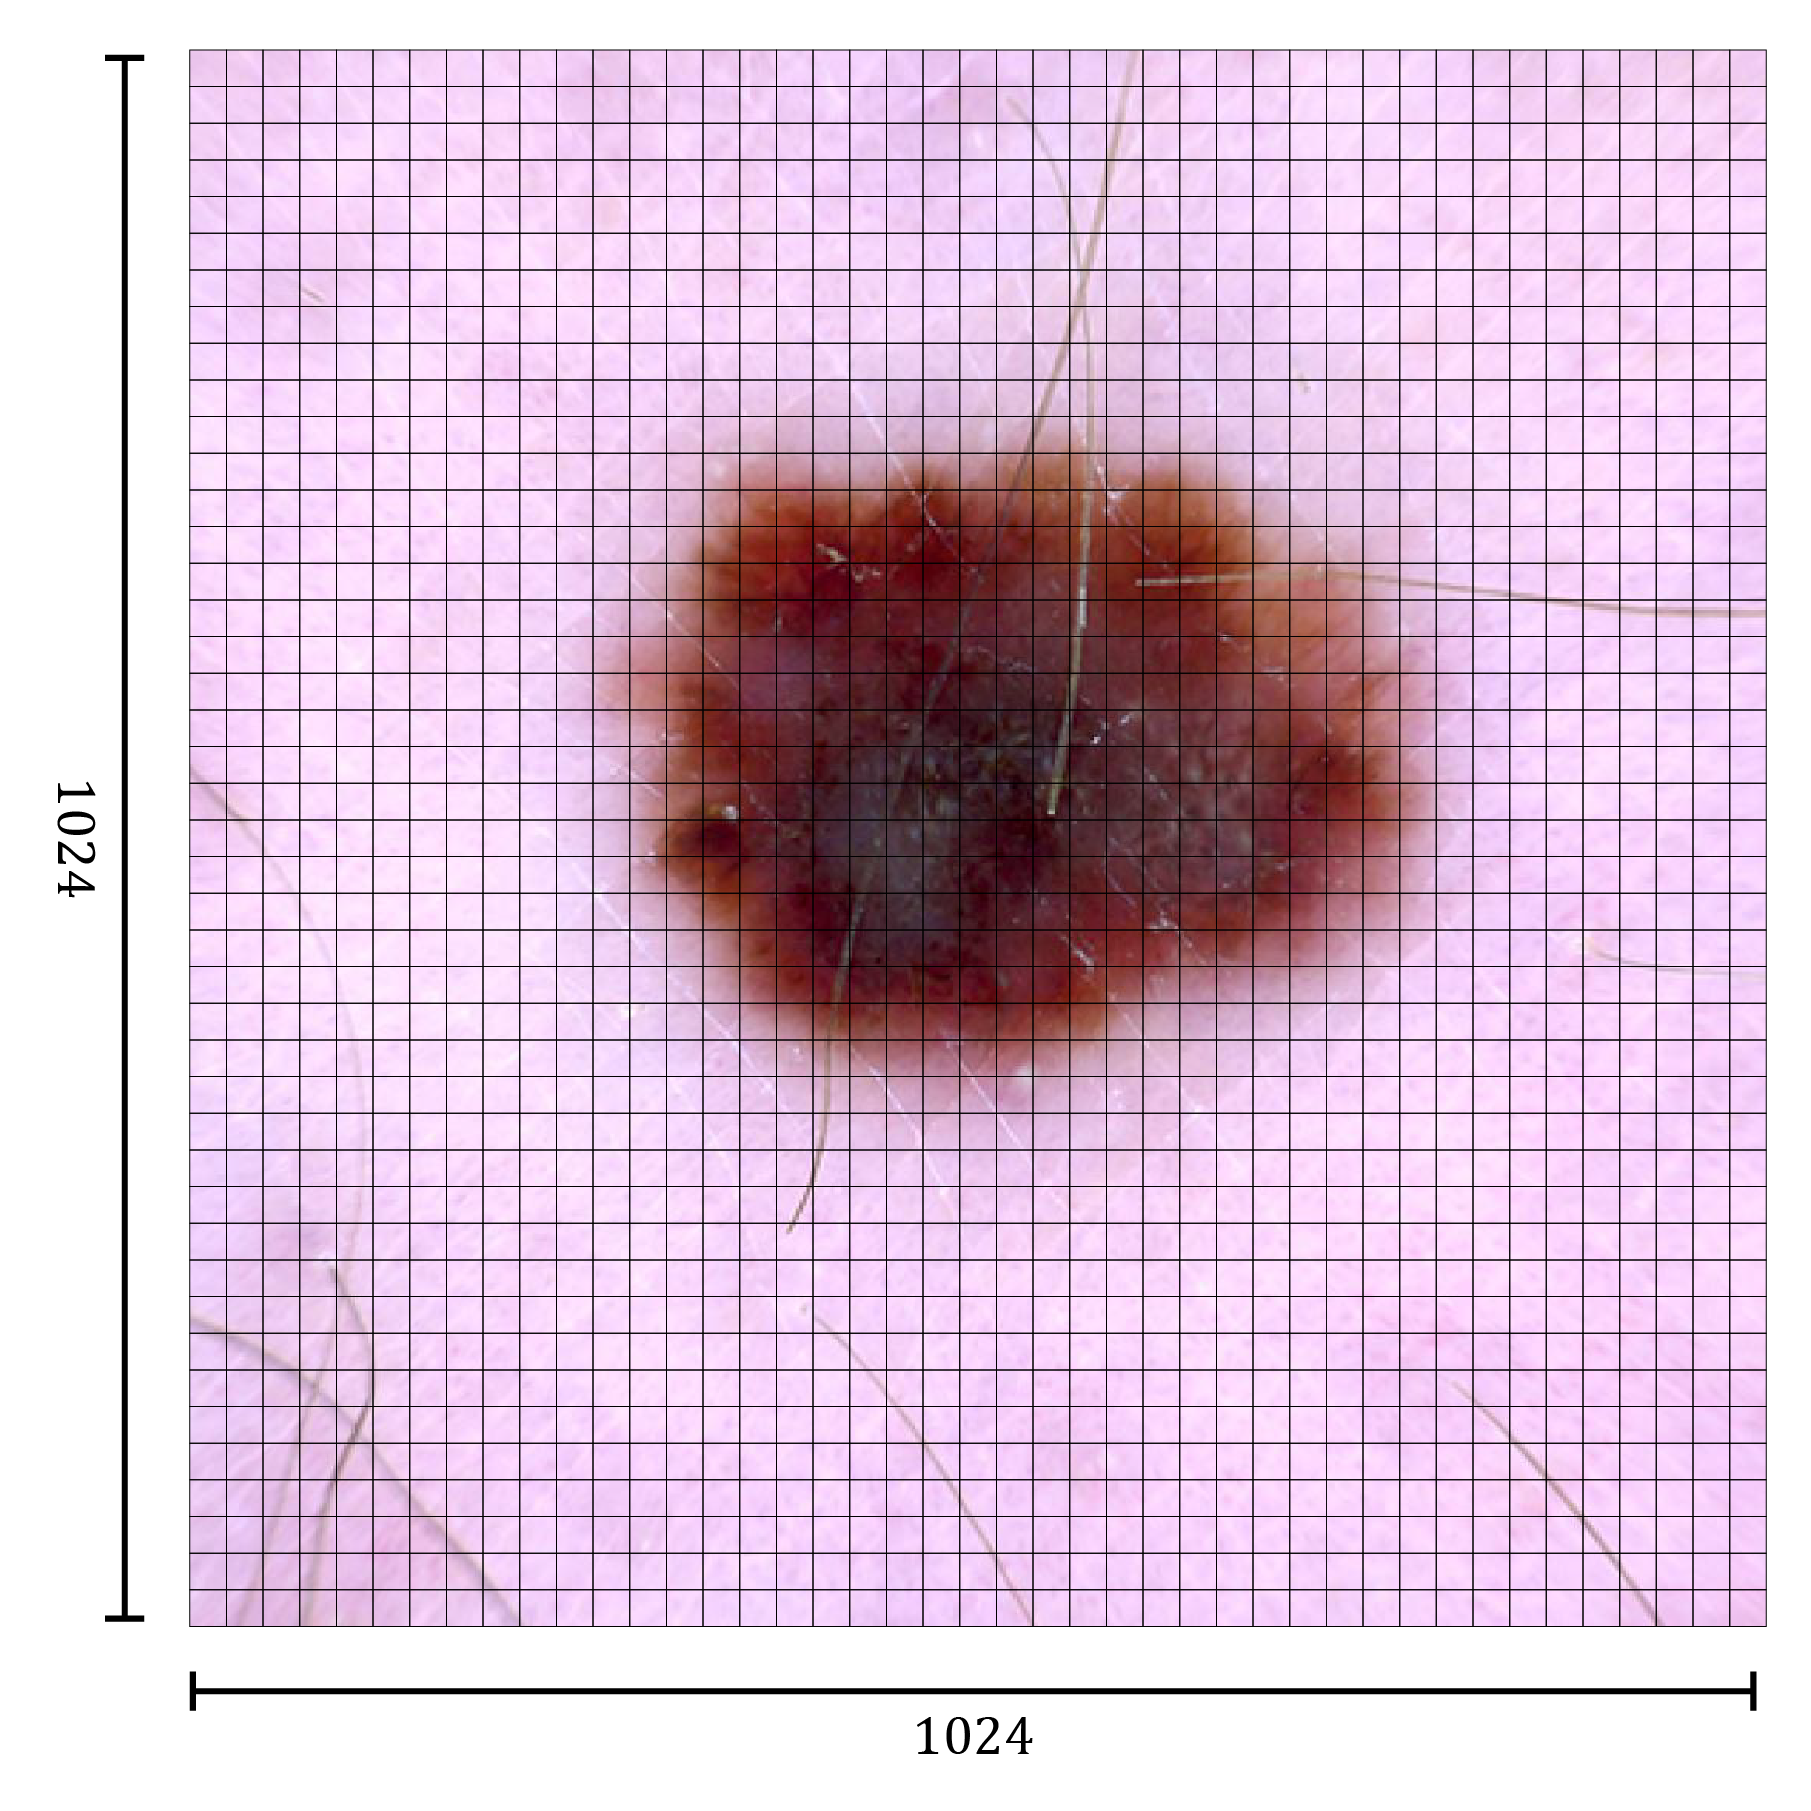
\includegraphics[width=5cm]{img/bab4/resize-1024.png}
            &
            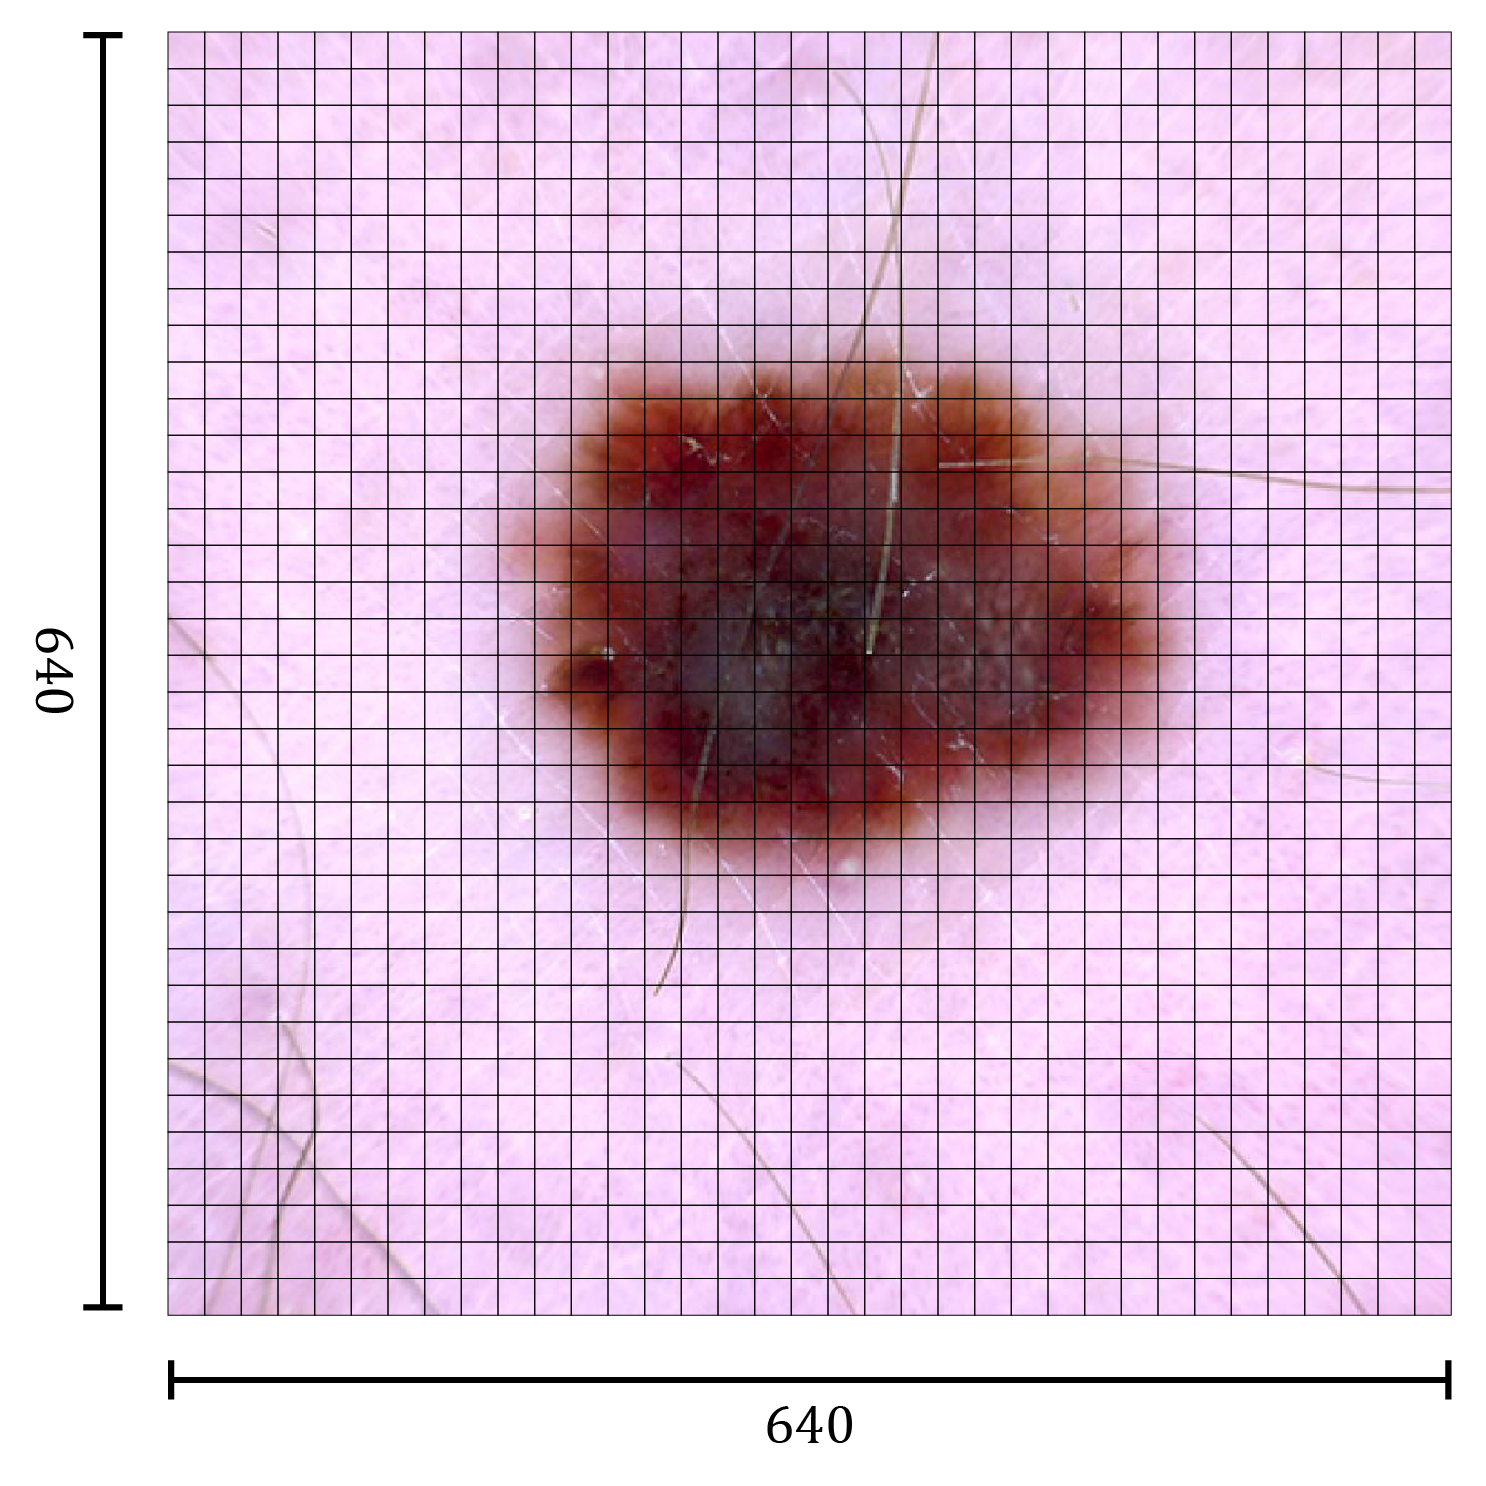
\includegraphics[width=5cm]{img/bab4/resize-640.png} \\
            (a)
            &
            (b) \\
        \end{tabular}
        \caption{\textit{Preprocessing} menggunakan \textit{resize} (a) Citra kanker kulit sebelum dilakukan \textit{resize}; (b) Citra kanker kulit setelah dilakukan \textit{resize}}
        \label{fig:d-resized}
    \end{figure}

    

    \subsection{\textit{Annotation}}
    \textit{Annotation} merupakan proses untuk memberikan label \textit{bounding box} pada citra. Hal ini berguna untuk memberikan informasi spasial mengenai objek yang ada pada citra sehingga YOLO dapat mempelajari dimana letak objek yang terdapat pada suatu citra. \textit{Annotation} dilakukan pada seluruh dataset sehingga dilakukan \textit{annotation} secara manual menggunakan Roboflow sebanyak 1600 citra. Gambar \ref{fig:d-annotation} memperlihatkan nilai yang dibutuhkan untuk melakukan proses \textit{annotation}.

    \begin{figure}[H]
        \centering
            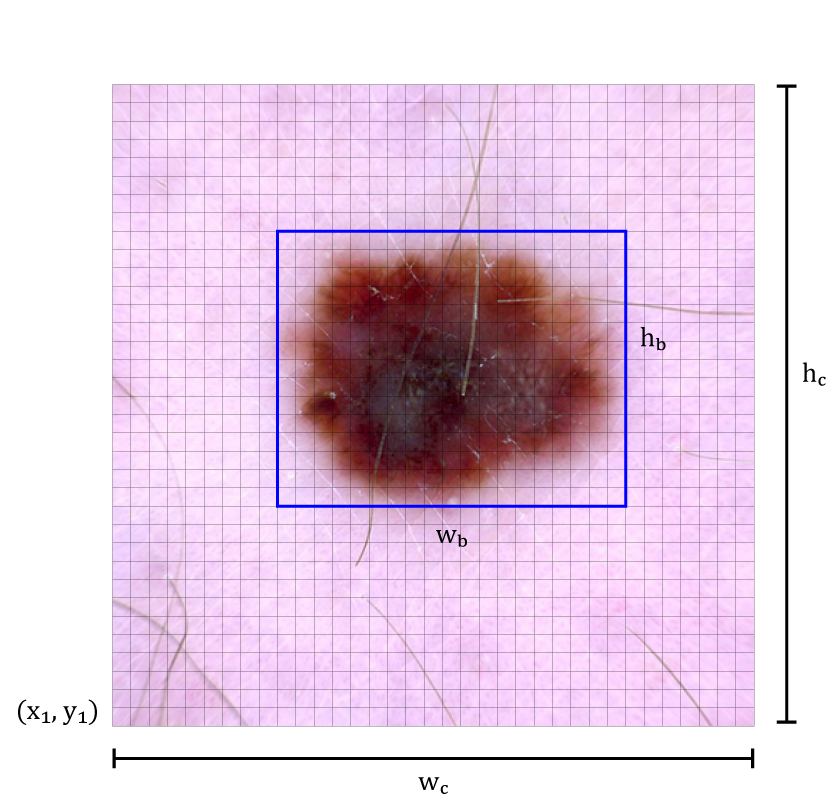
\includegraphics[width=5cm]{img/bab4/annotation.png}
        \caption{Ilustrasi proses \textit{annotation}}
        \label{fig:d-annotation}
    \end{figure}

    Berdasarkan Gambar \ref{fig:d-annotation}, \textit{annotation} dilakukan seperti perhitungan di bawah.

    \begin{alignat*}{5}
        (0) \Rightarrow x       &= \frac{x_1 + \frac{w_b}{2}}{w_c} \qquad\qquad &y  &=\frac{y_1 + \frac{h_b}{2}}{h_c}\\
                                &= \frac{110 + \frac{220}{2}}{640} \qquad\qquad &   &=\frac{80 + \frac{100}{2}}{640}\\
                                &= 0.34 \qquad\qquad                            &   &= 0.20\\
        w                       &= \frac{w_b}{w_c}\qquad\qquad                  &h  &= \frac{h_b}{h_c}\\
                                &= \frac{220}{640}\qquad\qquad                  &   &= \frac{100}{640}\\
                                &= 0.34\qquad\qquad                             &   &= 0.16\\
        (1) \Rightarrow x       &= \frac{x_1 + \frac{w_b}{2}}{w_c}\qquad\qquad  &y  &=\frac{y_1 + \frac{h_b}{2}}{h_c}\\
                                &= \frac{224 + \frac{300}{2}}{640}\qquad\qquad  &   &= \frac{155 + \frac{258}{2}}{640}\\
                                &= 0.58\qquad\qquad                             &   &= 0.44\\
        w                       &= \frac{w_b}{w_c}\qquad\qquad                  &h  &= \frac{h_b}{h_c}\\
                                &= \frac{300}{640}\qquad\qquad                  &   &= \frac{258}{640}\\
                                &= 0.47\qquad\qquad                             &   &= 0.40\\
        \vdots \\
        (1599) \Rightarrow x    &= \frac{x_1 + \frac{w_b}{2}}{w_c}\qquad\qquad  &y  &=\frac{y_1 + \frac{h_b}{2}}{h_c}\\
                                &= \frac{245 + \frac{172}{2}}{640}\qquad\qquad  &   &= \frac{180 + \frac{300}{2}}{640}\\
                                &= 0.58\qquad\qquad                             &   &= 0.50\\
        w                       &= \frac{w_b}{w_c}\qquad\qquad                  &h  &= \frac{h_b}{h_c}\\
                                &= \frac{172}{640}\qquad\qquad                  &   &= \frac{300}{640}\\
                                &= 0.27\qquad\qquad                             &   &= 0.47\\
    \end{alignat*}

    Pada perhitungan di atas, $(x, y)$ merepresentasikan nilai koordinat \textit{bounding box}, $w$ merepresentasikan lebar \textit{bounding box}, dan $h$ merepresentasikan tinggi \textit{bounding box}. Keempat nilai tersebut direpresentasikan dalam bentuk yang sudah dinormalisasi. Hasil dari proses \textit{annotation} seperti terlihat pada Tabel \ref{tab:d-annotation} dimana $c$ merepresentasikan kode kelas yang ada pada dataset.

    \begin{table}[H]
        \caption{\textit{Annotation}}
        \centering
        \begin{tabular}{cccccc}
            \hline
            Index       &$c$        &$x$        &$y$        &$w$        &$h$ \\ \hline
            $0$         &$5$        &$0.34$     &$0.20$     &$0.34$     &$0.16$ \\ \hline
            $1$         &$3$        &$0.58$     &$0.44$     &$0.47$     &$0.40$ \\ \hline
            $2$         &$1$        &$0.12$     &$0.24$     &$0.21$     &$0.21$ \\ \hline
            $3$         &$2$        &$0.63$     &$0.34$     &$0.61$     &$0.34$ \\ \hline
            $4$         &$7$        &$0.28$     &$0.24$     &$0.37$     &$0.30$ \\ \hline
            $\vdots$    &$\vdots$   &$\vdots$   &$\vdots$   &$\vdots$   &$\vdots$ \\ \hline
            $1599$      &$2$        &$0.58$     &$0.50$     &$0.27$     &$0.47$ \\ \hline
        \end{tabular}
        \label{tab:d-annotation}
    \end{table}

\section{Pelatihan Model}
Setelah proses \textit{preprocessing}, citra akan masuk ke tahap \textit{feature learning} dan \textit{object detection} sehingga mendapatkan model terbaik atau bisa disebut proses pelatihan model. Model terbaik didapatkan dari beberapa percobaan yang dilakukan pada proses pelatihan model. Penelitian ini melakukan beberapa percobaan untuk mendapatkan model terbaik. Terdapat tiga jenis percobaan, yaitu uji coba model YOLOv7, uji coba \textit{batch size}, dan uji coba \textit{epochs}. Penelitian ini melakukan uji coba versi YOLOv7, yaitu YOLOv7 dan YOLOv7 Tiny dengan mempertimbangkan waktu komputasi yang dibutuhkan untuk mendapatkan model yang optimal karena YOLOv7 Tiny masih mempertahankan arsitektur YOLOv4 dan memiliki arsitektur yang tidak lebih kompleks daripada YOLOv7. Hal ini akan sangat mempengaruhi waktu komputasi. \textit{Batch size} juga dilakukan uji coba untuk mendapatkan nilai yang optimal dengan akurasi tinggi pada proses pelatihan model. Penelitian ini menggunakan beberapa nilai \textit{batch size}, yaitu 32, 64, dan 128. Uji coba terakhir pada penelitian ini, yaitu \textit{epochs} dengan mempertimbangkan waktu komputasi dan akurasi yang meningkat seiring bertambahnya \textit{epochs}. Penelitian ini menggunakan beberapa nilai \textit{epochs}, yaitu 300, 600, dan 1200.
    \subsection{\textit{Convolutional Layer}}
    Sebagian besar arsitektur YOLOv7 tersusun dari \textit{convolutional layer} seperti terlihat pada Gambar \ref{fig:yolov7-archi}. Setiap operasi konvolusi pada YOLOv7 dilengkapi dengan \textit{Batch Normalization} dan fungsi aktivasi \textit{Sigmoid-weighted Linear Unit}. Pada \textit{convolutiona layer} terjadi proses pembelajaran fitur dari citra masukan dan \textit{feature map} dengan \textit{filter} yang ada pada YOLOv7. YOLOv7 menggunakan 3 operasi konvolusi dengan komposisi yang berbeda pada ukuran \textit{filter} ($f$) dan jumlah \textit{stride} ($s$), yaitu operasi konvolusi dengan $f=1\times 1$ dan $s=1$, $f=3\times 3$ dan $s=1$, $f=3\times 3$ dan $s=2$. Nilai $f$ dan $s$ ditentukan oleh arsitektur YOLOv7. Sedangkan \textit{padding} $(p)$ pada seluruh \textit{convolutional layer} di YOLOv7 bernilai 1 kecuali \textit{maxpool layer} yang tidak menggunakan \textit{padding}. Nilai yang ada pada \textit{filter} ditentukan secara acak oleh arsitektur YOLOv7 yang terdiri dari 3 lapisan sesuai dengan data masukan yang berupa citra RGB dengan 3 kanal. Contoh perhitungan \textit{convolutional layer} menggunakan data masukan citra RGB kanker kulit berukuran $640\times 640$ dengan 32 \textit{filter} berukuran $3\times 3$ pada masing-masing kanal RGB seperti terlihat pada Gambar \ref{fig:d-convol}.

    \begin{figure}[H]
        \centering
            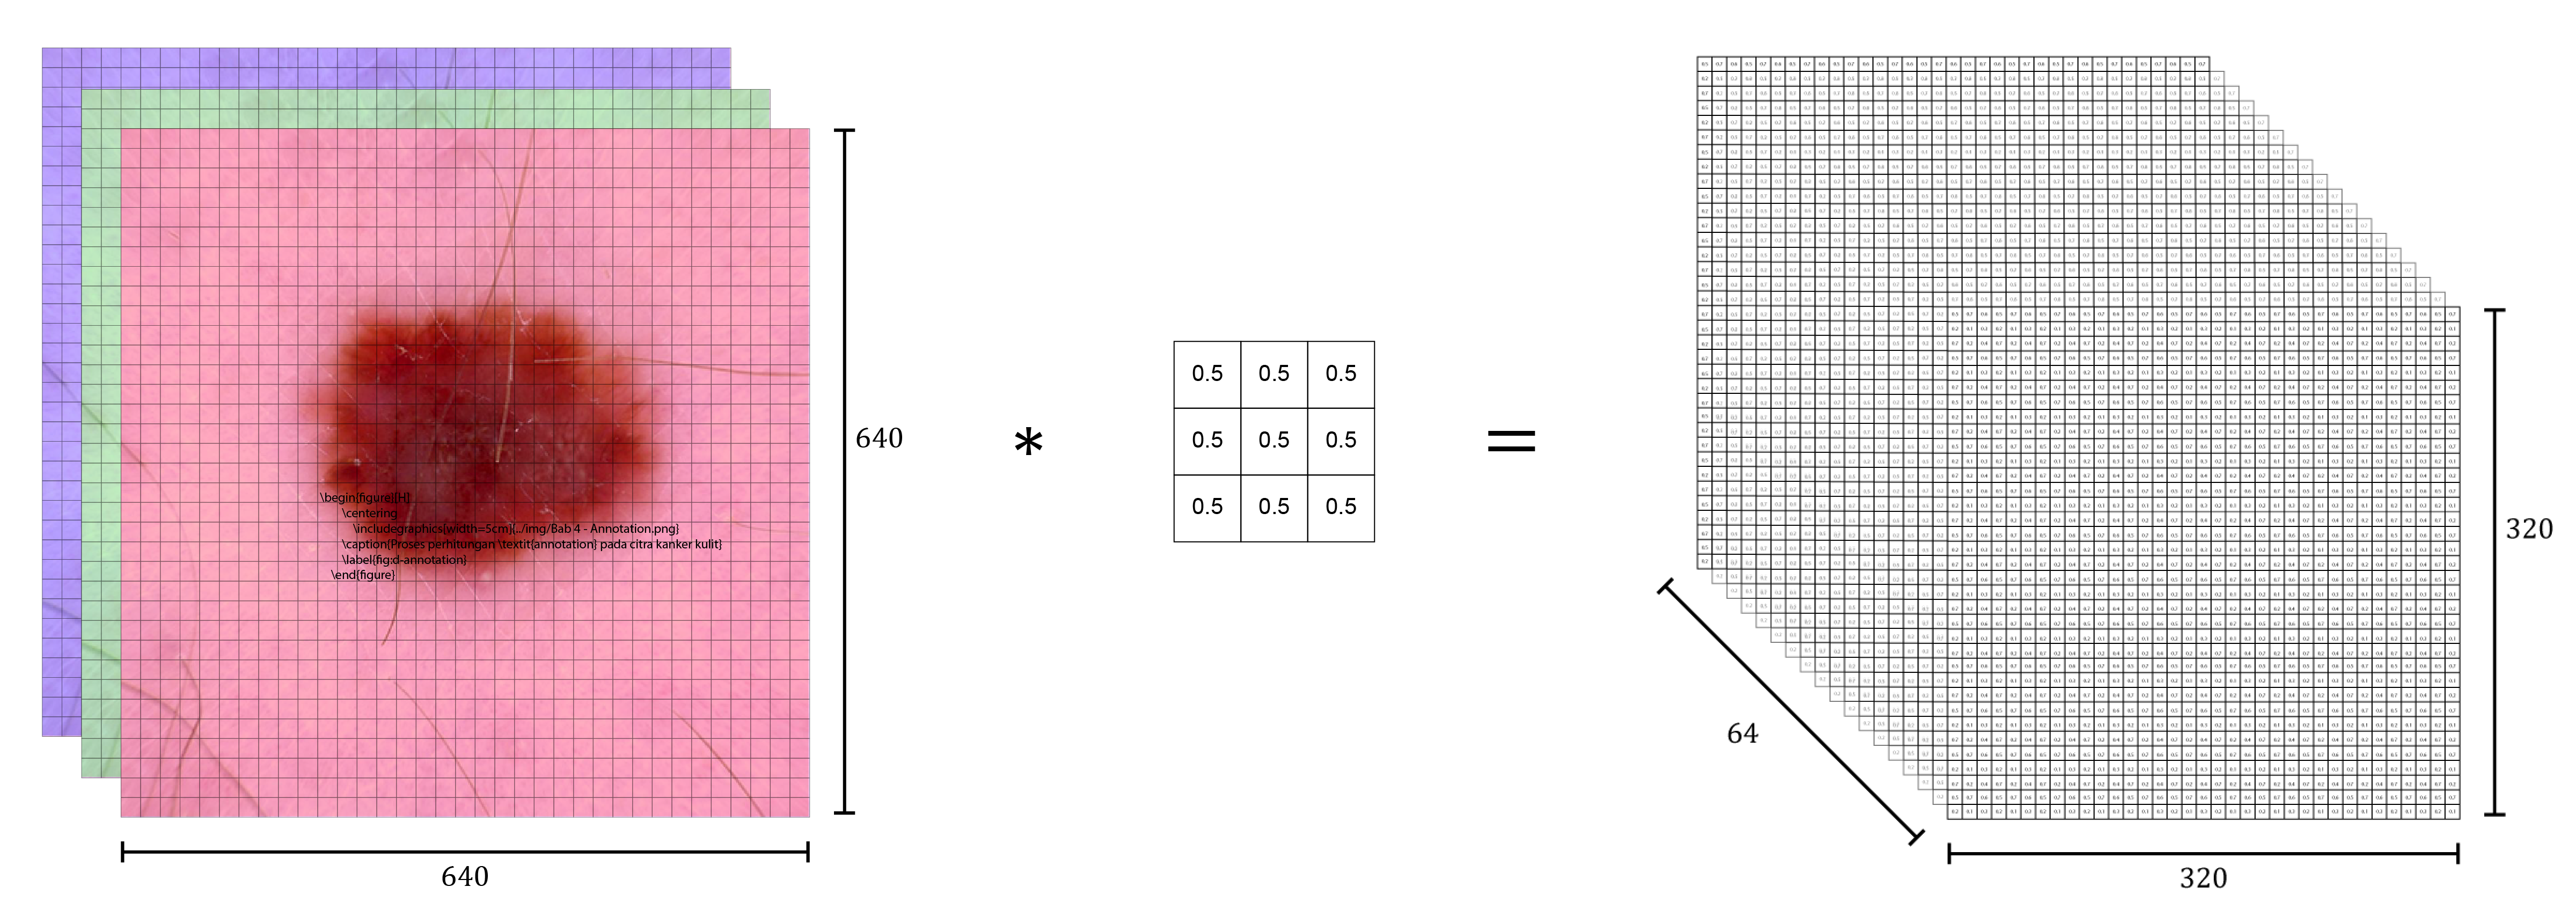
\includegraphics[width=10cm]{img/bab4/convolution.png}
        \caption{Ilustrasi operasi konvolusi data masukan dengan \textit{filter} yang menghasilkan \textit{feature map}}
        \label{fig:d-convol}
    \end{figure}

    Seperti terlihat pada Gambar \ref{fig:d-convol}, operasi konvolusi antara data masukan dengan \textit{filter} yang sudah ditentukan oleh YOLOv7 akan menghasilkan \textit{feature map}. Pada \textit{convolution layer} pertama, YOLOv7 menggunakan ukuran \textit{filter} $3\times 3$ dengan $s=1$. Ukuran dan dimensi dari \textit{feature map} dapat dihitung sesuai dengan perhitungan di bawah ini.

    \begin{align*}
        w &= \frac{w - f + 2p}{s} + 1\\
        &= \frac{640 - 3 + 2(1)}{1} + 1\\
        &= 640
    \end{align*}

    Perhitungan di atas memperlihatkan bahwa ukuran \textit{feature map} dari operasi konvolusi data masukan berukuran $640\times 640$ terhadap \textit{filter} berukuran $3\times 3$ dengan $s=1$ dan $p=1$ menghasilkan \textit{feature map} berukuran $640\times 640$ piksel. Pada arsitektur YOLOv7 seperti terlihat pada Gambar \ref{fig:yolov7-archi}, \textit{layer} pertama pada YOLOv7 menghasilkan 32 \textit{feature map} dengan ukuran $640\times 640$ piksel. Ilustrasi perhitungan operasi konvolusi data masukan dengan \textit{filter} pada \textit{layer} pertama di YOLOv7 dapat dicontohkan seperti di bawah ini.

    \begin{alignat*}{5}
        R_{(0, 0)}          &=  &&\bigl( I_{r}(0, 0)\times F_{r}(0, 0) + I_{r}(0, 1)\times F_{r}(0, 1) + I_{r}(0, 2)\times F_{r}(0, 2) + \cdots + \\
                            &   &&I_{r}(2, 2)\times F_{r}(2, 2) \bigr) + \bigl( I_{g}(0, 0)\times F_{g}(0, 0) + I_{g}(0, 1)\times F_{g}(0, 1) + \\
                            &   &&I_{g}(0, 2)\times F_{g}(0, 2) + \cdots + I_{g}(2, 2)\times F_{g}(2, 2) \bigr) + \bigl( I_{b}(0, 0)\times F_{b}(0, 0) + \\
                            &   &&I_{b}(0, 1)\times F_{b}(0, 1) + I_{b}(0, 2)\times F_{b}(0, 2) + \cdots + I_{b}(2, 2)\times F_{b}(2, 2) \bigr) \\
        % === Batas rumus
                            &=  &&\bigl( (0.925490\times 0.19116) + (0.925490\times 0.17358) + (0.925490\times \\
                            &   &&0.17896) + \cdots + (0.913725\times 0.13184) \bigr) + \bigl( (0.776471\times 0.19116) + \\
                            &   &&(0.776471\times 0.17358) + (0.776471\times 0.17896) + \cdots + (0.764706\times \\
                            &   &&0.13184) \bigr) + \bigl( (0.937255\times 0.19116) + (0.937255\times 0.17358) + \\
                            &   &&(0.937255\times 0.17896) + \cdots + (0.925490\times 0.13184) \bigr) \\
                            &=  &&0.404922 \\
        \vdots \\
        R_{(639, 639)}      &=  &&\bigl( I_{r}(638, 638)\times F_{r}(638, 638) + I_{r}(638, 639)\times F_{r}(638, 639) + \\
                            &   &&I_{r}(638, 640)\times F_{r}(638, 640) + \cdots + I_{r}(640, 640)\times F_{r}(640, 640) \bigr) + \\
                            &   &&\bigl( I_{g}(638, 638)\times F_{g}(638, 638) + I_{g}(638, 639)\times F_{g}(638, 639) + \\
                            &   &&I_{g}(638, 640)\times F_{g}(638, 640) + \cdots + I_{g}(640, 640)\times F_{g}(640, 640) \bigr) + \\
                            &   &&\bigl( I_{b}(638, 638)\times F_{b}(638, 638) + I_{b}(638, 639)\times F_{b}(638, 639) + \\
                            &   &&I_{b}(638, 640)\times F_{b}(638, 640) + \cdots + I_{b}(640, 640)\times F_{b}(640, 640) \bigr) \\
        % === Batas Rumus
                            &=  &&\bigl( (0.941176\times 0.19116) + (0.945098\times 0.17358) + (0.937255\times \\
                            &   &&0.17896) + \cdots + (0.949020\times 0.13184) \bigr) + \bigl( (0.760784\times 0.19116) + \\
                            &   &&(0.764706\times 0.17358) + (0.756863\times 0.17896) + \cdots + (0.768627\times \\
                            &   &&0.13184) \bigr) + \bigl( (0.941176\times 0.19116) + (0.945098\times 0.17358) + \\
                            &   &&(0.937255\times 0.17896) + \cdots + (0.949020\times 0.13184) \bigr) \\
                            &=  &&0.258519 \\
    \end{alignat*}

    Perhitungan di atas akan menghasilkan \textit{feature map} hasil dari operasi data masukan dengan \textit{filter} sebagaimana matriks di bawah ini. Matriks di bawah adalah salah satu dari 32 \textit{feature map} dengan ukuran $640\times 640$ yang dihasilkan dari operasi konvolusi pada perhitungan di atas.

    \begin{align*}
        R_{(:, :, 0)} = 
        \begin{pmatrix}
            0.404922 & 0.445536 & 0.445536 & 0.445536 & \cdots & 0.458136 \\
            0.349199 & 0.309777 & 0.309777 & 0.309777 & \cdots & 0.326002 \\
            0.348241 & 0.309294 & 0.309294 & 0.309294 & \cdots & 0.326987 \\
            0.348800 & 0.310123 & 0.310123 & 0.310123 & \cdots & 0.340638 \\
            0.350666 & 0.311744 & 0.311837 & 0.311837 & \cdots & 0.337295 \\
            \vdots   & \vdots   & \vdots   & \vdots   & \ddots &\vdots \\
            0.265303 & 0.246458 & 0.250151 & 0.255221 & \cdots & 0.258519 \\
        \end{pmatrix}_{640\times 640}
    \end{align*}

    Visualisasi 32 \textit{feature map} hasil dari operasi konvolusi pada perhitungan di atas seperti terlihat pada Gambar \ref{fig:d-feamap}.

    \begin{figure}[H]
        \begin{center}
            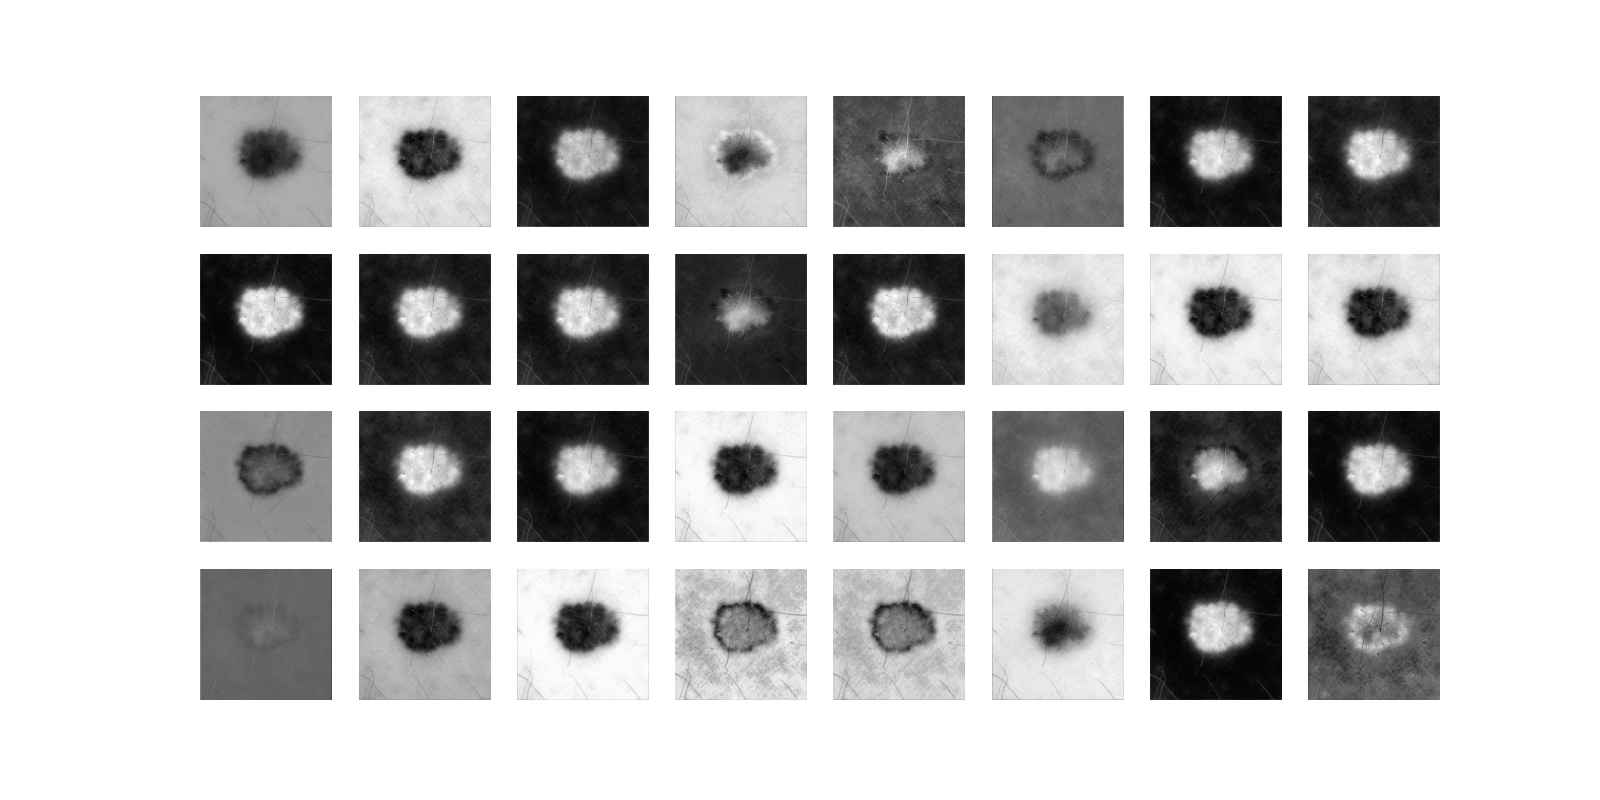
\includegraphics[width=12cm]{img/bab4/conv-layer.png}
            \caption{Visualisasi \textit{feature map} pada YOLOv7}
            \label{fig:d-feamap}
        \end{center}
    \end{figure}
    
    \subsection{\textit{Batch Normalization}}

    Setelah mendapatkan hasil \textit{feature map}, YOLOv7 mengubah \textit{feature map} tersebut ke dalam bentuk yang dinormalisasi dengan menggunakan \textit{batch normalization}. Perhitungan \textit{batch normalization} dilakukan menggunakan Persamaan \ref{eq:bn-4} dimana $\mu = -0.002345$, $\sigma^2 = 29.41072$, $\epsilon = 0.001$, $\gamma = 1.0021$, dan $\beta = 1.624$. Perhitungan \textit{batch normalization} seperti terlihat di bawah.

    \begin{align*}
        \breve{Z}_{0, 0}     &= \gamma \left( \frac{Z_{i} - \mu}{\sqrt{\sigma^2 - \epsilon}} \right) + \beta \\
                             &= 1.0021 \left( \frac{0.404922 - (-0.002345)}{\sqrt{29.41072 - 0.001}} \right) + 1.624\\
                             &= -0.589056\\
        \vdots\\
        \breve{Z}_{639, 639} &= \gamma \left( \frac{Z_{i} - \mu}{\sqrt{\sigma^2 - \epsilon}} \right) + \beta \\
                             &= 1.0021 \left( \frac{0.258519 - (-0.002345)}{\sqrt{29.41072 - 0.001}} \right) + 1.624\\
                             &= -5.816965\\
    \end{align*}

    Hasil perhitungan masing-masing nilai untuk \textit{batch normalization} seperti terlihat pada matriks di bawah ini.

    \begin{align*}
        R_{(:, :, 0)} = 
        \begin{pmatrix}
            -0.589056 & 0.861231  & 0.861231  & 0.861231  & \cdots & -0.807409 \\
            -2.578891 & -3.986590 & -3.986590 & -3.986590 & \cdots & -2.776101 \\
            -2.613092 & -4.003831 & -4.003831 & -4.003831 & \cdots & -2.778702 \\
            -2.593120 & -3.974232 & -3.974232 & -3.974232 & \cdots & -2.884571 \\
            -2.526499 & -3.916370 & -3.913023 & -3.913023 & \cdots & -3.003972 \\
            \vdots    & \vdots    & \vdots    & \vdots    & \ddots & \vdots \\
            -5.574710 & -6.247649 & -6.115799 & -5.934733 & \cdots & -5.816965 \\
        \end{pmatrix}_{640\times 640}
    \end{align*}

    Nilai pada \textit{feature map} hasil normalisasi memiliki interval yang tidak terlalu jauh seperti terlihat pada matriks di atas. Visualisasi \textit{feature map} yang telah melewati \textit{batch normalization layer} seperti terlihat pada Gambar \ref{fig:d-banorm}.

    \begin{figure}[H]
        \begin{center}
            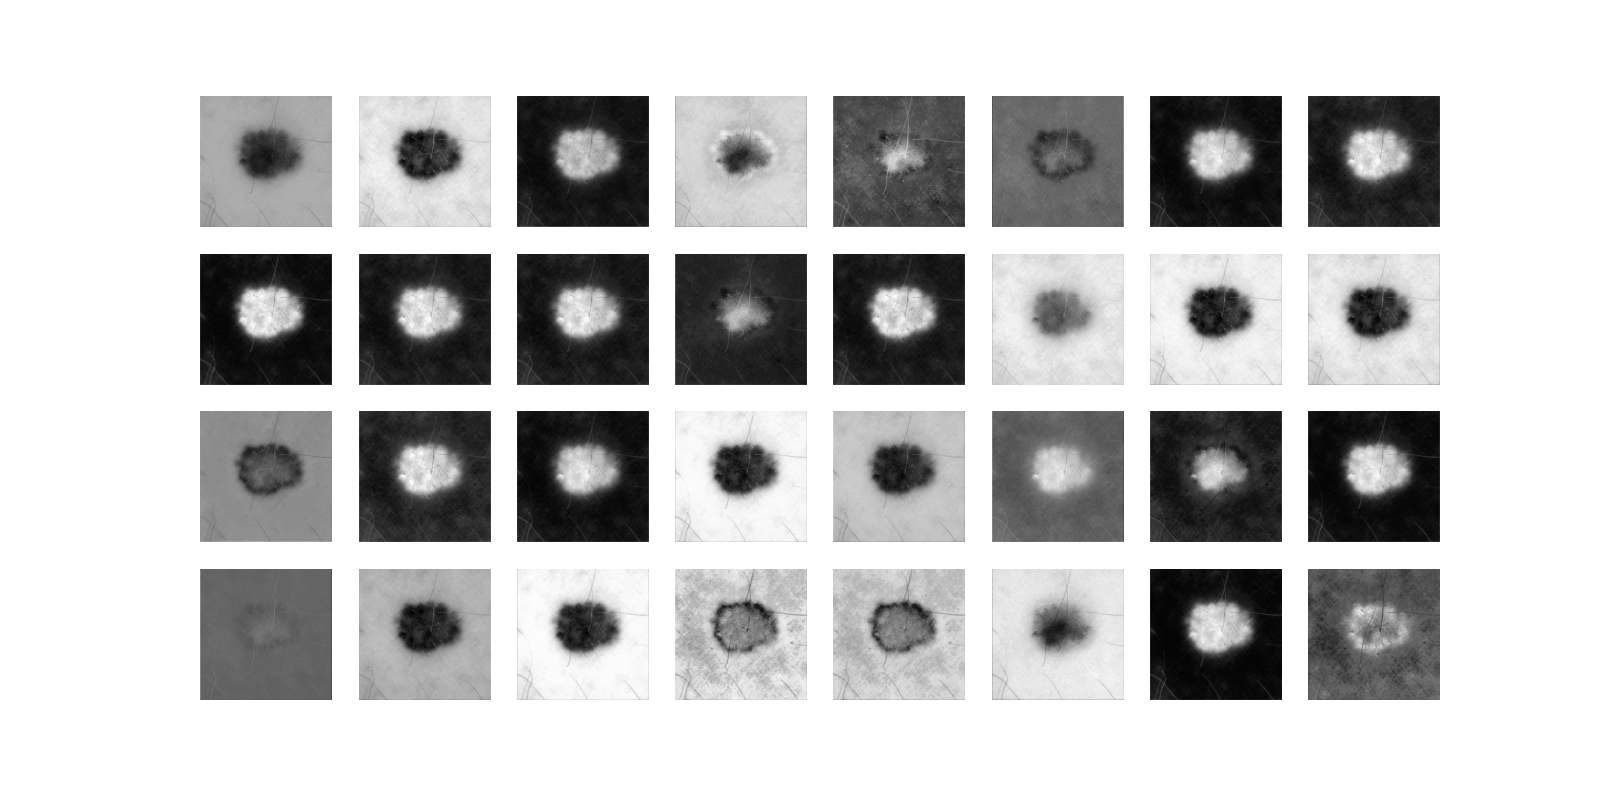
\includegraphics[width=12cm]{img/bab4/bn-layer.png}
            \caption{Visualisasi \textit{feature map} setelah melewati \textit{batch normalization layer} pada YOLOv7}
            \label{fig:d-banorm}
        \end{center}
    \end{figure}

    \subsection{\textit{Leaky Rectified Linear Unit} (Leaky ReLU)}

    YOLOv7 Tiny menggunakan Leaky ReLU untuk fungsi aktivasi pada setiap \textit{layer} di arsitekturnya. Hal ini akan mengurangi waktu komputasi jika dibandingkan dengan fungsi aktivasi SiLU. Fungsi aktivasi Leaky ReLU menerima sedikit nilai negatif dengan grafik menaik secara konstan seperti terlihat pada Gambar \ref{fig:l-relu}. Perhitungan fungsi aktivasi Leaky ReLU menggunakan Persamaan \ref{eq:l-relu} seperti terlihat di bawah ini.

    \begin{align*}
        f(x)_{(0, 0)}       &= max(0.1\times x, x) \\
                            &= max(0.1\times (-0.589056), -0.589056) \\
                            &= max(0.1\times (-0.589056), -0.589056) \\
                            &= -0.005891 \\
        \vdots \\
        f(x)_{(639, 639)}   &= max(0.1\times x, x) \\
                            &= max(0.1\times (-5.816965), -5.816965) \\
                            &= max(0.1\times (-5.816965), -5.816965) \\
                            &= -0.058170 \\
    \end{align*}

    Hasil \textit{feature map} yang telah diaktivasi menggunakan Leaky ReLU seperti terlihat di bawah ini.

    \begin{align*}
        R_{(:, :, 0)} = 
        \begin{pmatrix}
            -0.005891 & 0.861231  & 0.861231  & 0.861231  & \cdots & -0.008074 \\
            -0.025789 & -0.039866 & -0.039866 & -0.039866 & \cdots & -0.027761 \\
            -0.026131 & -0.040038 & -0.040038 & -0.040038 & \cdots & -0.027787 \\
            -0.025931 & -0.039742 & -0.039742 & -0.039742 & \cdots & -0.028846 \\
            -0.025265 & -0.039164 & -0.039130 & -0.039130 & \cdots & -0.030040 \\
            \vdots    & \vdots    & \vdots    & \vdots    & \ddots & \vdots \\
            -0.055747 & -0.062476 & -0.061158 & -0.059347 & \cdots & -0.058170 \\
        \end{pmatrix}_{640\times 640}
    \end{align*}

    Perhitungan fungsi aktivasi Leaky ReLU terjadi hingga pada \textit{feature map} terakhir. Visualisasi \textit{feature map} yang telah melewati fungsi aktivasi Leaky ReLU seperti terlihat pada Gambar \ref{fig:d-lrelu}.

    \begin{figure}[H]
        \begin{center}
            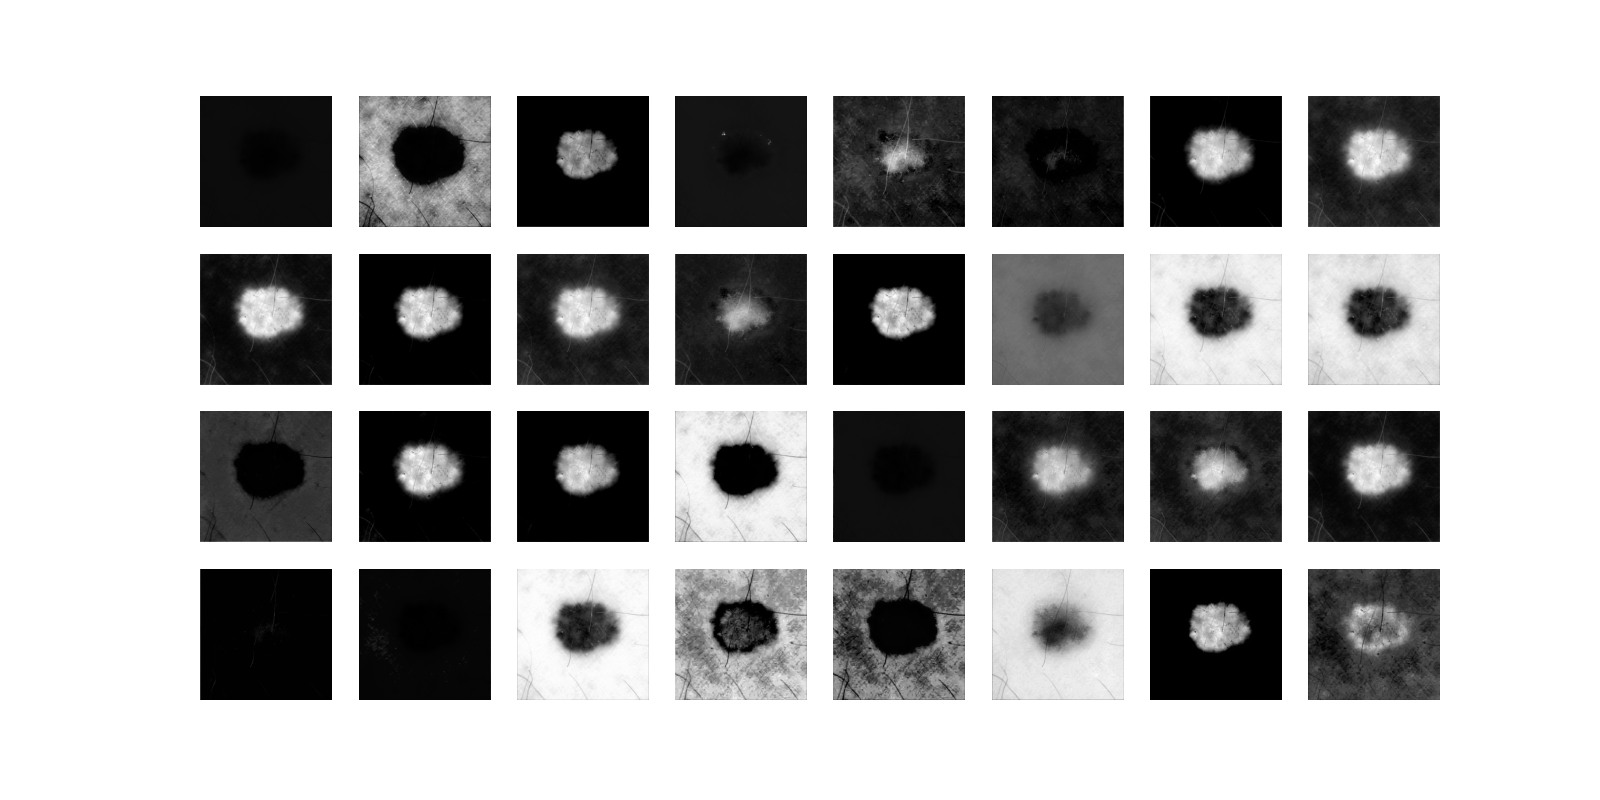
\includegraphics[width=12cm]{img/bab4/lrelu-layer.png}
            \caption{Visualisasi \textit{feature map} setelah melewati fungsi aktivasi Leaky ReLU pada YOLOv7}
            \label{fig:d-lrelu}
        \end{center}
    \end{figure}

    \subsection{\textit{Sigmoid-weighted Linear Unit} (SiLU)}
    Peningkatan yang paling utama dari YOLOv7 adalah fungsi aktivasi SiLU. Hal ini juga meningkatkan waktu komputasi karena fungsi aktivasi SiLU memiliki persamaan yang lebih kompleks daripada fungsi aktivasi Leaky ReLU. Dapat dilihat pada Gambar \ref{fig:silu} bahwa grafik terlihat menaik dengan tidak konstan. Meskipun hal ini meningkatkan waktu komputasi, namun SiLU dapat meningkatkan akurasi pada YOLOv7. Perhitungan fungsi aktivasi SiLU menggunakan Persamaan \ref{eq:silu} seperti terlihat di bawah ini.

    \begin{align*}
        a_k(z_k)_{(0, 0)}       &= z_k\frac{1}{1+e^{-(z_k)}} \\
                                &= -0.589056\frac{1}{1+2.718^{0.589056}} \\
                                &= -0.210206 \\
        \vdots \\
        a_k(z_k)_{(319, 319)}   &= z_k\frac{1}{1+e^{-(z_k)}} \\
                                &= -5.816965\frac{1}{1+2.718^{5.816965}} \\
                                &= -0.017264 \\
    \end{align*}

    Hasil \textit{feature map} yang telah melewati fungsi aktivasi SiLU seperti terlihat pada matriks di bawah ini.

    \begin{align*}
        R_{(:, :, 0)} = 
        \begin{pmatrix}
            -0.210206 & 0.605375  & 0.605375  & 0.605375  & \cdots & -0.249040 \\
            -0.181836 & -0.072654 & -0.072654 & -0.072654 & \cdots & -0.162761 \\
            -0.178476 & -0.071743 & -0.071743 & -0.071743 & \cdots & -0.162515 \\
            -0.180436 & -0.073313 & -0.073313 & -0.073313 & \cdots & -0.152656 \\
            -0.187015 & -0.076465 & -0.076651 & -0.076651 & \cdots & -0.141928 \\
            \vdots    & \vdots    & \vdots    & \vdots    & \ddots & \vdots \\
            -0.021063 & -0.012066 & -0.013472 & -0.015661 & \cdots & -0.017264 \\
        \end{pmatrix}_{320\times 320}
    \end{align*}

    Perhitungan fungsi aktivasi SiLU terjadi hingga pada lapisan terakhir. Visualisasi \textit{feature map} yang telah melewati fungsi aktivasi Silu seperti terlihat pada Gambar \ref{fig:d-silu}.

    \begin{figure}[H]
        \begin{center}
            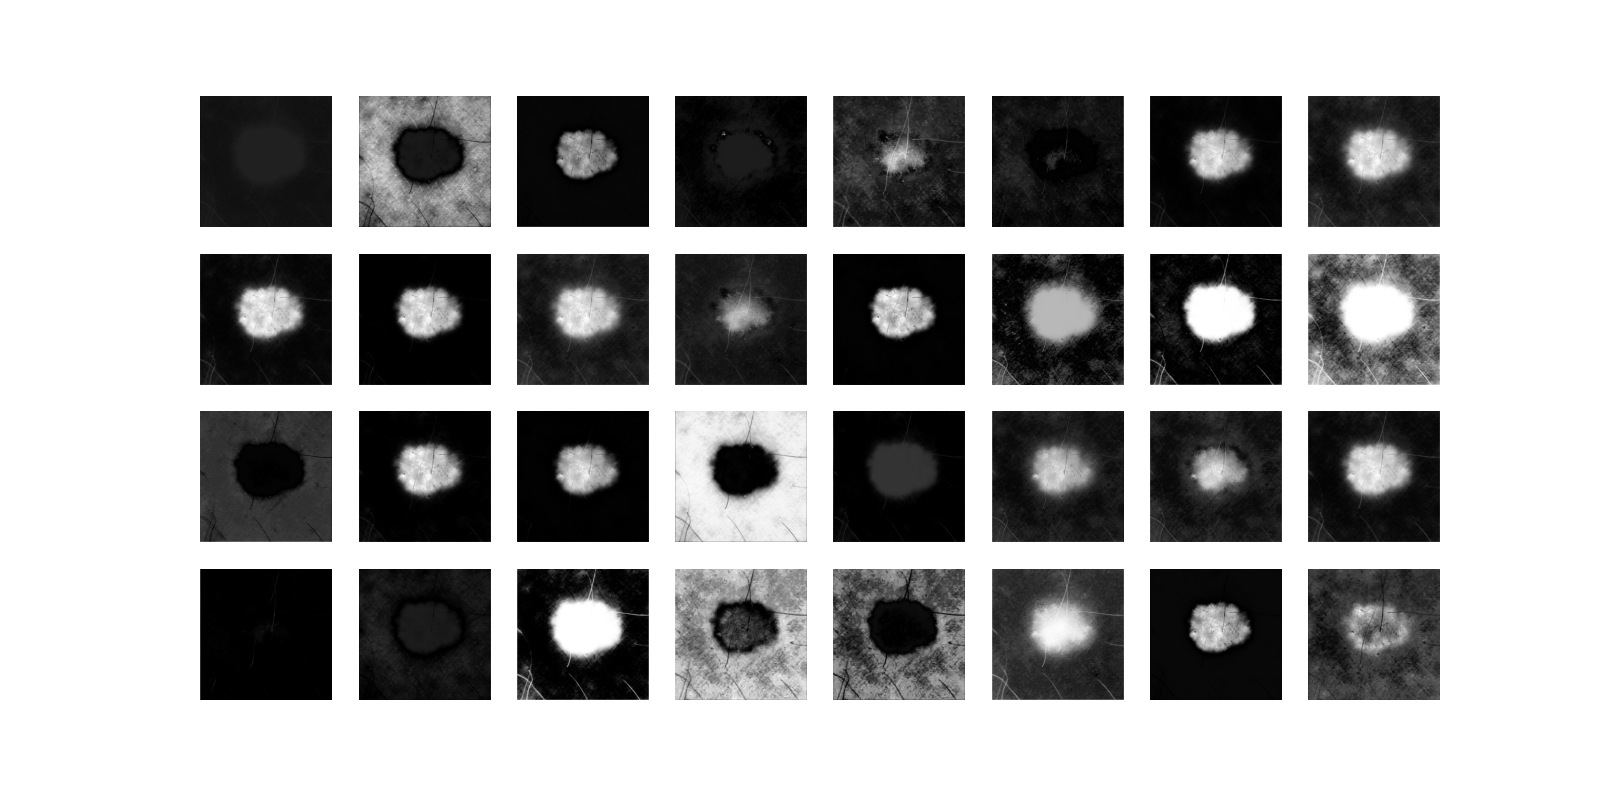
\includegraphics[width=12cm]{img/bab4/silu-layer.png}
            \caption{Visualisasi \textit{feature map} setelah melewati fungsi aktivasi SiLU pada YOLOv7}
            \label{fig:d-silu}
        \end{center}
    \end{figure}

    \subsection{\textit{Pooling Layer}}

    \textit{Pooling layer} berguna untuk mengurangi ukuran \textit{feature map} sehingga dapat mempercepat waktu komputasi pada saat pelatihan model YOLOv7. \textit{Pooling layer} mengurangi ukuran pada masing-masing \textit{feature map} tanpa menghilangkan informasi yang penting dari \textit{feature map}. Arsitektur YOLOv7 menggunakan \textit{max-pooling} dimana \textit{max-pooling} mengambil nilai maksimum pada ukuran \textit{filter} tertentu. Arsitektur YOLOv7 menggunakan ukuran \textit{filter} $2\times 2$ untuk mengimplementasikan \textit{pooling layer}. Berdasarkan hasil \textit{feature map} fungsi aktivasi SiLU, perhitungan \textit{pooling layer} untuk setiap nilainya seperti terlihat di bawah ini.

    \begin{align*}
        P_{(0, 0)}      &= max(-0.210206, 0.605375, -0.181836, -0.072654)\\
                        &= 0.605375 \\
        \vdots \\
        P_{(319, 319)}  &= max(-0.087075, -0.128279, -0.017056, -0.017264)\\
                        &= -0.128279 \\
    \end{align*}

    Hasil \textit{feature map} setelah melewati \textit{pooling layer} seperti terlihat di bawah ini.

    \begin{align*}
        R_{(:, :, 0)} = 
        \begin{pmatrix}
            0.605375  & -0.143407 & -0.139577 & -0.148889 & \cdots & -0.221489 \\
            -0.185320 & -0.084338 & -0.053553 & -0.076679 & \cdots & -0.146808 \\
            -0.206630 & -0.090965 & -0.077647 & -0.070564 & \cdots & -0.187663 \\
            -0.201531 & -0.089601 & -0.077569 & -0.064958 & \cdots & -0.194047 \\
            -0.202485 & -0.085817 & -0.061791 & -0.076593 & \cdots & -0.189475 \\
            \vdots    & \vdots    & \vdots    & \vdots    & \ddots & \vdots \\
            -0.192949 & -0.270050 & -0.256753 & -0.253126 & \cdots & -0.128279 \\
        \end{pmatrix}_{80, 80}
    \end{align*}

    Visualisasi \textit{feature map} yang telah melewati \textit{max-pooling layer} seperti terlihat pada Gambar \ref{fig:d-maxpool}.

    \begin{figure}[H]
        \begin{center}
            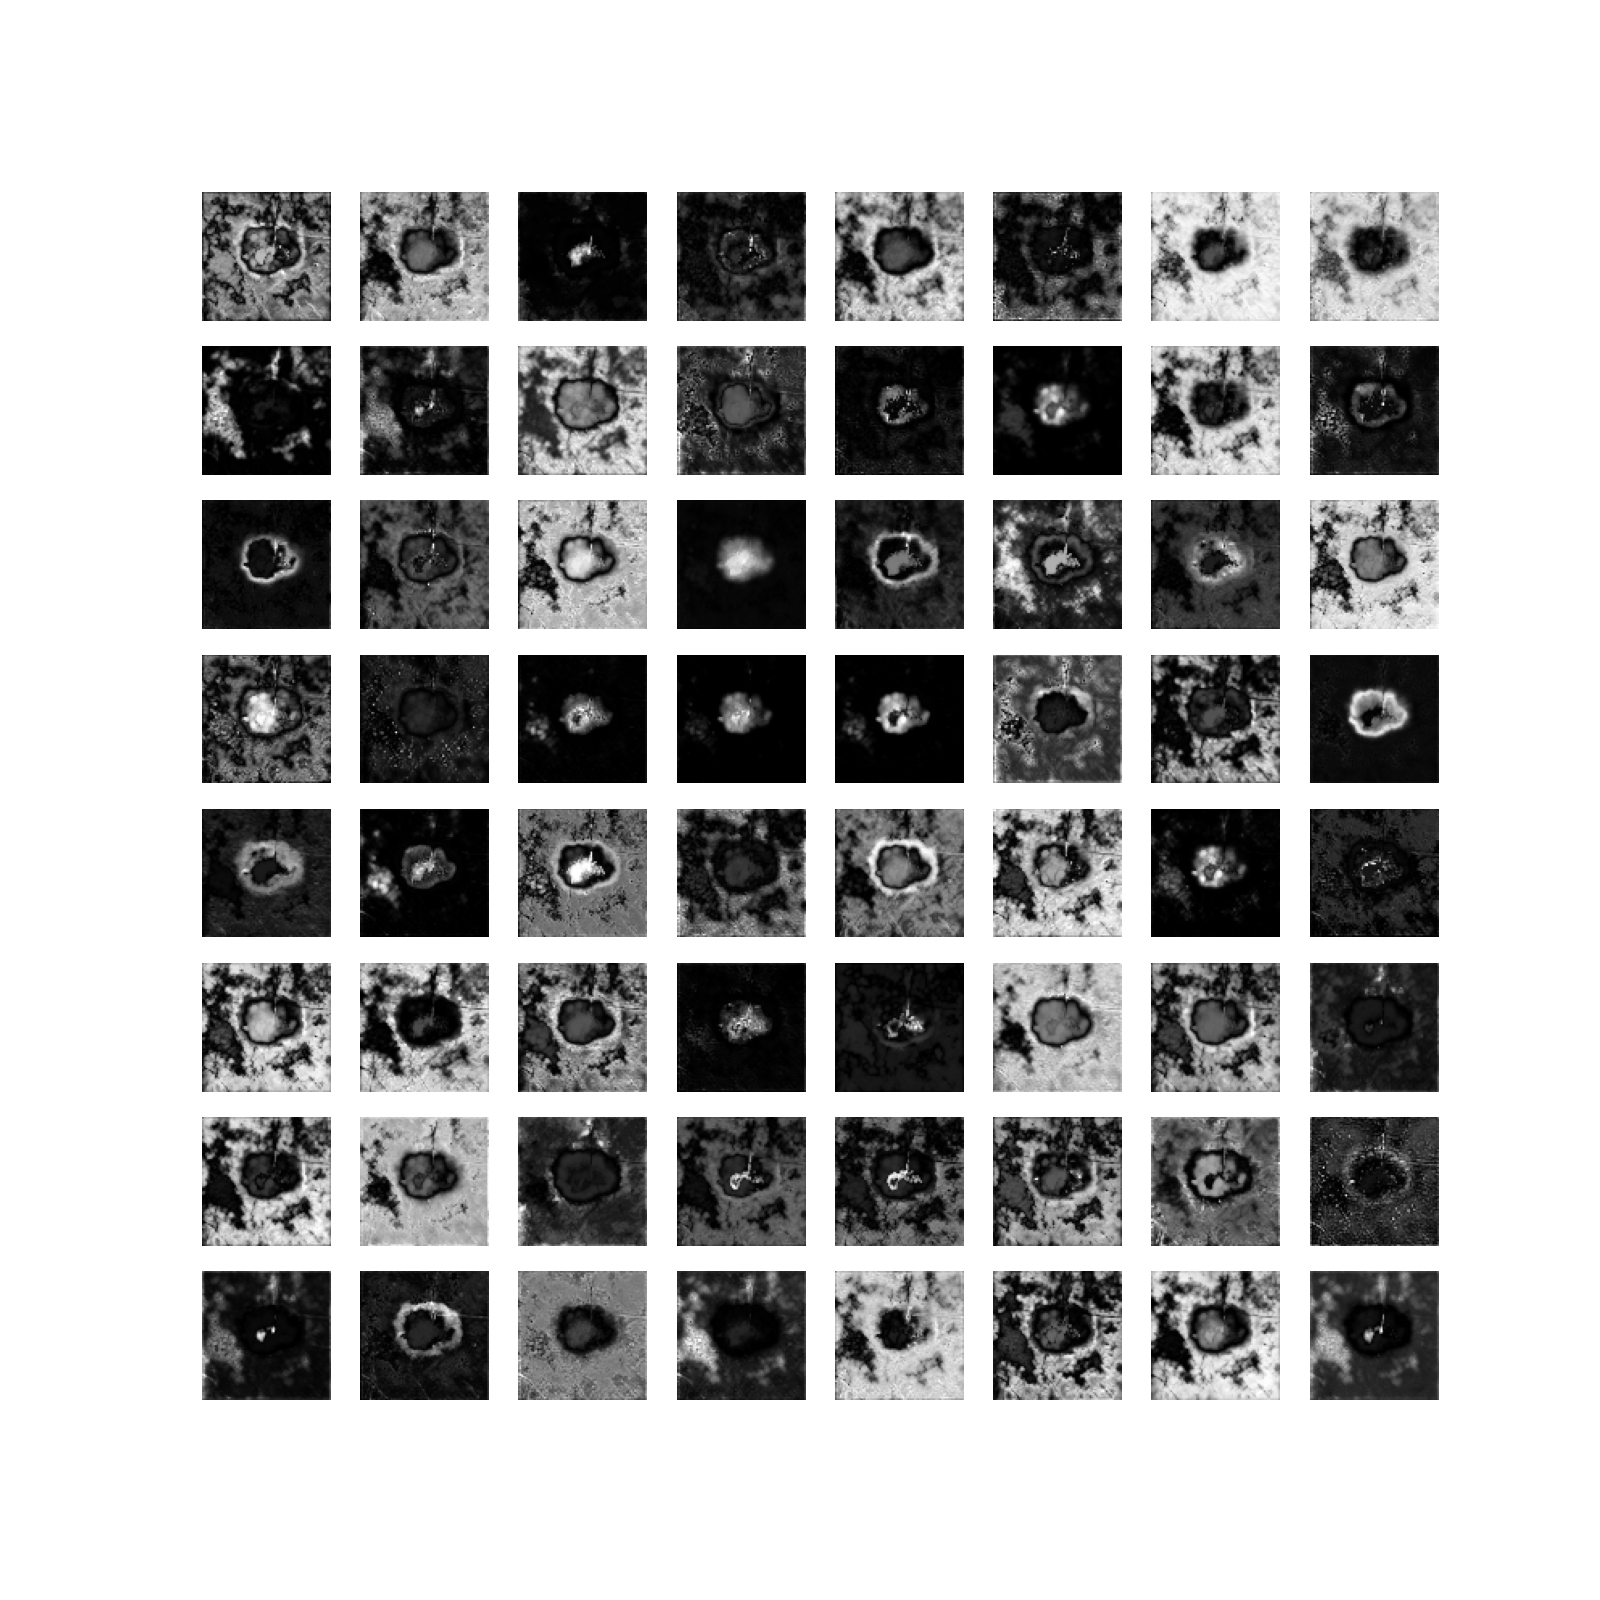
\includegraphics[width=12cm]{img/bab4/mp-layer.png}
            \caption{Visualisasi \textit{feature map} setelah melewati \textit{max-pooling layer} pada YOLOv7}
            \label{fig:d-maxpool}
        \end{center}
    \end{figure}

    \subsection{\textit{Upsample Layer}}

    Proses untuk mengembalikan ukuran \textit{feature map} dapat dilakukan menggunakan \textit{upsample layer}. \textit{Upsample layer} mengembalikan ukuran \textit{feature map} seperti pada ukuran sebelumnya. \textit{Unpooling layer} adalah nama lain dari \textit{upsample layer}. Sehingga, \textit{upsample layer} dapat diimplementasikan setelah \textit{feature map} melewati \textit{downsample layer} atau \textit{pooling layer} untuk mengurangi waktu komputasi. Perhitungan \textit{upsample layer} pada YOLOv7 menggunakan metode \textit{nearest} atau mempertimbangkan nilai piksel di sekitarnya untuk melakukan \textit{upsample}. Ilustrasi \textit{upsample layer} seperti terlihat pada Gambar \ref{fig:il-nearest}. \textit{Upsample layer} pada arsitektur YOLOv7 terletak setelah banyak proses konvolusi dan \textit{max-pool} sehingga \textit{feature map} yang telah melewati \textit{upsample layer} memiliki ukuran $40\times 40$ seperti di bawah ini.

    \begin{align*}
        R_{(40, 40, 0)} = 
        \begin{pmatrix}
            -0.240868 & -0.240868 & -0.240287 & -0.240287 & \cdots & -0.238043 \\
            -0.240868 & -0.240868 & -0.240287 & -0.240287 & \cdots & -0.238043 \\
            -0.244172 & -0.244172 & -0.240042 & -0.240042 & \cdots & -0.240131 \\
            -0.244172 & -0.244172 & -0.240042 & -0.240042 & \cdots & -0.240131 \\
            -0.251152 & -0.251152 & -0.236841 & -0.236841 & \cdots & -0.256989 \\
            \vdots    & \vdots    & \vdots    & \vdots    & \ddots & \vdots \\
            -0.262205 & -0.262205 & -0.264320 & -0.264320 & \cdots & -0.242232 \\
        \end{pmatrix}
    \end{align*}

    Visualisasi \textit{feature map} yang telah melewati \textit{upsample layer} seperti terlihat pada Gambar \ref{fig:d-uplayer}.

    \begin{figure}[H]
        \begin{center}
            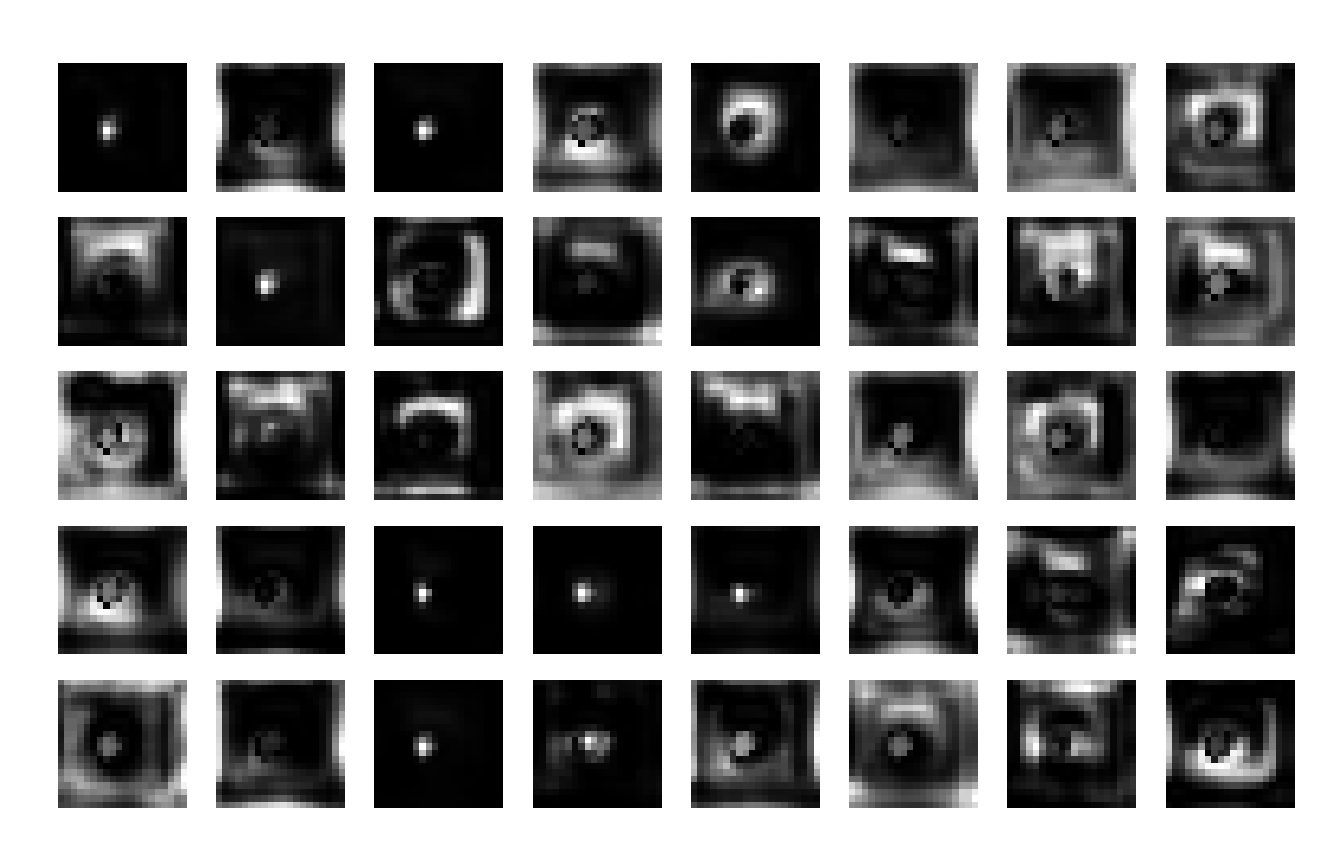
\includegraphics[width=12cm]{img/bab4/up-layer.png}
            \caption{Visualisasi \textit{feature map} setelah melewati \textit{upsample layer} pada YOLOv7}
            \label{fig:d-uplayer}
        \end{center}
    \end{figure}

    \subsection{\textit{Efficient Layer Aggregation Networks (ELAN)}}

    Pada YOLOv7, terdapat 8 jaringan ELAN dengan struktur masing-masing menggunakan \textit{Convolutional Layer}, \textit{Batch Normalization}, dan \textit{Sigmoid-weighted Linear Unit} (CBS). Jaringan ELAN memiki operasi konvolusi yang bertumpuk hingga pada layer terakhir digabungkan dengan hasil keluaran dari layer awal sehingga meningkatkan pembelajaran fitur pada YOLOv7. ELAN terdiri dari $2\times CBS$ di bagian awal untuk mengurangi dimensi \textit{feature map} karena menggunakan ukuran \textit{filter} $1\times 1$ dengan $s = 1$. Kemudian terdapat 4 \textit{layer} untuk pembelajaran fitur menggunakan filter berukuran \textit{filter} $3\times 1$ dengan $s = 1$. Pada bagian akhir struktur ELAN, terdapat \textit{Concatenation Layer} yang berguna untuk menggabungkan semua hasil pembelajaran fitur pada \textit{layer} sebelumnya sehingga menghasilkan \textit{feature map} baru. Visualisasi \textit{feature map} yang telah melewati jaringan \textit{ELAN} seperti terlihat pada Gambar \ref{fig:d-elan}.

    \begin{figure}[H]
        \begin{center}
            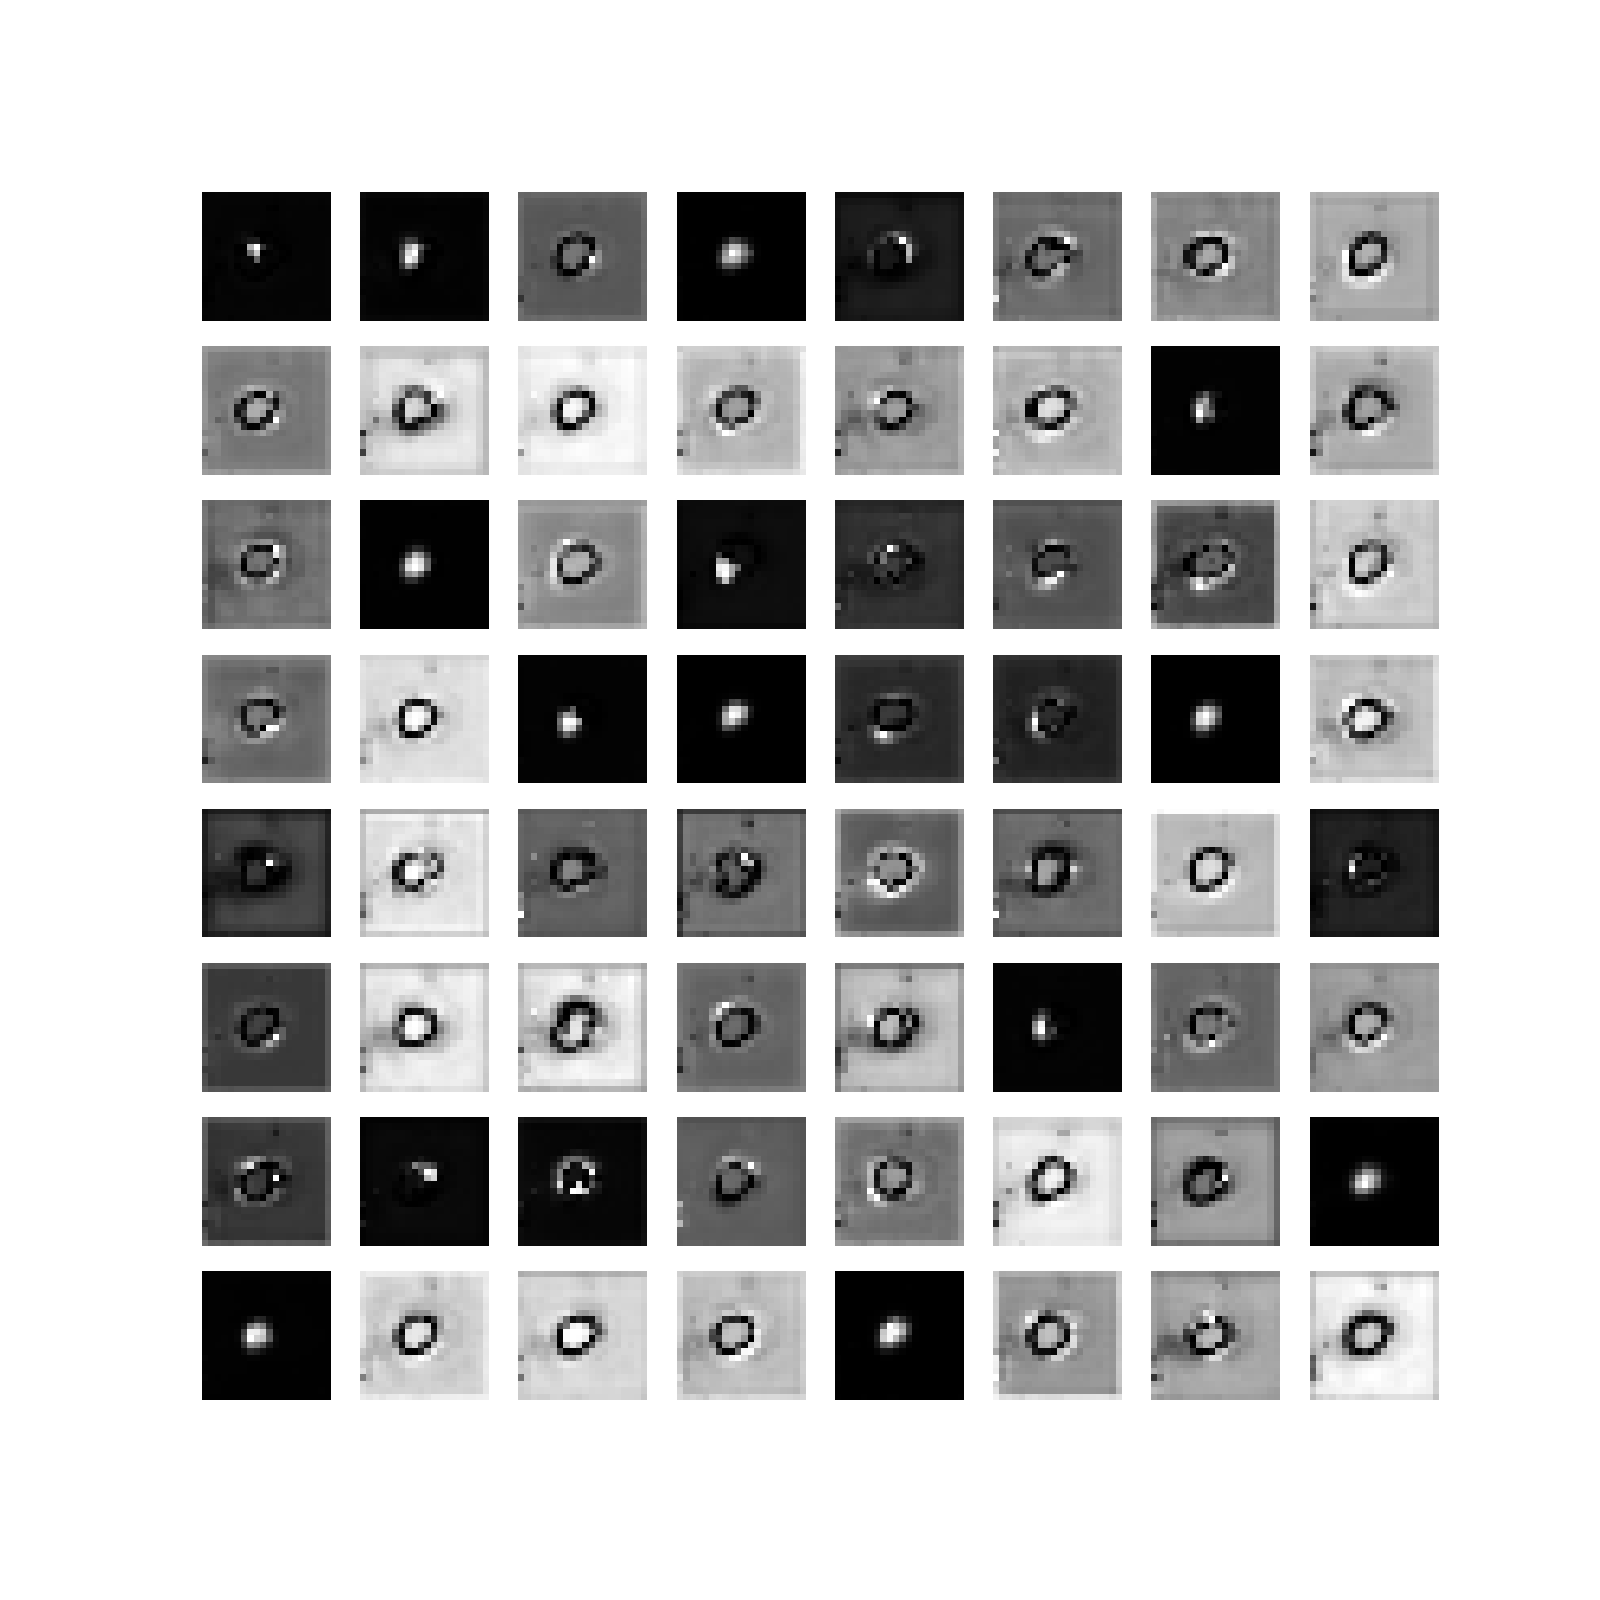
\includegraphics[width=12cm]{img/bab4/elan-layer.png}
            \caption{Visualisasi \textit{feature map} setelah melewati jaringan \textit{ELAN} pada YOLOv7}
            \label{fig:d-elan}
        \end{center}
    \end{figure}

    \subsection{\textit{Intesection over Union} (IoU)}
    YOLOv7 menggunakan IoU untuk mengetahui keakuratan hasil prediksi model yang telah dilakukan pelatihan model. Hasil prediksi model yang berupa tumpukan \textit{feature map} atau tensor dilakukan pengukuran keakuratan \textit{bounding box} yang telah diprediksi menggunakan IoU terhadap \textit{ground truth}. \textit{Ground truth} merupakah data aktual yang telah diberikan label berupa jenis kanker dan \textit{bounding box}. Perhitungan IoU memerlukan informasi terkait \textit{overlap area} dan \textit{union area} yang dihitung menggunakan Persamaan \ref{eq:oa} dan \ref{eq:ua}. Contoh perhitungan IoU menggunakan Persamaan \ref{eq:iou} seperti terlihat di bawah ini.

    \begin{align*}
        x_{a1} &= max(3, 5)\\
               &= 5\\
        y_{a1} &= max(4, 10)\\
               &= 10\\
        x_{a2} &= min(13, 17)\\
               &= 13\\
        y_{a2} &= min(15, 19)\\
               &= 15\\
        OA     &= (13-5)\times (15-10)\\
               &= 40\\
        UA     &= (13-3)\times (15-4) + (17-5)\times (19-10) - 40\\
               &= 178\\
        IoU    &= \frac{40}{178}\\
               &= 0.224
    \end{align*}

    Seperti terlihat pada perhitungan di atas, nilai IoU 0.224 merupakan nilai yang kecil karena mendekati 0. Jika nilai ambang batas yang diberikan adalah 0.5 maka hasil prediksi termasuk ke dalam FP.

\section{Pengujian dan Evaluasi Sistem}
Tingkat keberhasilan model klasifikasi jenis kanker kulit menggunakan YOLOv7 dipengaruhi oleh beberapa faktor terkait metode yang diimplementasikan, antara lain varian metode, ukuran \textit{batch size}, dan \textit{epochs}. Sehingga, penelitian ini melakukan beberapa uji coba untuk mendapatkan model terbaik dengan mempertimbangkan perangkat yang dipakai, yaitu $2\times GPU T100$ dengan total GPU \textit{memory} 30gb. Mempertimbangkan hal tersebut, penelitian ini melakukan uji coba varian YOLOv7, yaitu YOLOv7 dan YOLOv7 Tiny. Pada uji coba \textit{batch size}, penelitian ini menggunakan nilai 32, 64, dan 128. Kemudian uji coba \textit{epochs} dilakukan menggunakan nilai 300, 600, dan 1200. Model terbaik dipilih dengan mempertimbangkan nilai mAP pada semua kelas.

Penelitian ini menggunakan \textit{kaggle notebook} untuk melakukan pelatihan model YOLOv7 sehingga penelitian ini memiliki batas sumber daya dan waktu komputasi sehingga terdapat beberapa uji coba yang tidak bisa diselesaikan. Hal ini memengaruhi uji coba \textit{batch size} pada YOLOv7 sehingga uji coba yang awalnya menggunakan nilai \textit{batch size} 32, 64, dan 128 diubah menjadi 16, 32, dan 40. Meskipun penelitian ini mengurangi nilai \textit{batch size} pada YOLOv7, terdapat uji coba yang tidak dapat terselesaikan, yaitu uji coba YOLOv7 dengan 16 \textit{batch size} dan 1200 \textit{epochs}. Hal ini terjadi karena \textit{runtime} GPU pada \textit{kaggle notebook} maksimal hingga 12 jam. Sedangkan waktu pelatihan model YOLOv7 dengan 16 \textit{batch size} dan 1200 \textit{epochs} melebihi batas waktu 12 jam. Hasil uji coba klasifikasi kanker kulit menggunakan YOLOv7 seperti terlihat pada Tabel \ref{tab:d-testing}.

\begin{table}[H]
    \caption{Hasil uji coba varian YOLOv7, \textit{batch size} dan \textit{epochs} pada penelitian ini}
    \centering
    \begin{tabular}{|c|c|c|c|c|c|c|}
        \hline
        Varian YOLO                  & \textit{Batch Size}  & \textit{Epochs} & \textit{Time (h)}  & P     & R     & mAP\\
        \hline
        \multirow{8}{*}{YOLOv7}      & \multirow{2}{*}{16}  & 300             & 5.847              & 0.632 & 0.656 & 0.661\\ \cline{3-7}
                                     &                      & 600             & 11.755             & 0.752 & 0.769 & 0.778\\ \cline{2-7}
                                     & \multirow{3}{*}{32}  & 300             & 3.439              & 0.699 & 0.693 & 0.715\\ \cline{3-7}
                                     &                      & 600             & 6.806              & 0.776 & 0.606 & 0.695\\ \cline{3-7}
                                     &                      & 1200            & 11.423             & 0.773 & 0.720 & 0.749\\ \cline{2-7}
                                     & \multirow{3}{*}{40}  & 300             & 3.225              & 0.725 & 0.678 & 0.696\\ \cline{3-7}
                                     &                      & 600             & 6.692              & 0.775 & 0.626 & 0.694\\ \cline{3-7}
                                     &                      & 1200            & 11.308             & 0.784 & 0.727 & 0.773\\ \cline{2-7}
        \hline
        \multirow{9}{*}{YOLOv7 Tiny} & \multirow{3}{*}{32}  & 300             & 1.683              & 0.851 & 0.662 & 0.782\\ \cline{3-7}
                                     &                      & 600             & 3.521              & 0.709 & 0.644 & 0.689\\ \cline{3-7}
                                     &                      & 1200            & 7.084              & 0.785 & 0.804 & 0.827\\ \cline{2-7}
                                     & \multirow{3}{*}{64}  & 300             & 1.731              & 0.752 & 0.757 & 0.789\\ \cline{3-7}
                                     &                      & 600             & 3.409              & 0.640 & 0.600 & 0.635\\ \cline{3-7}
                                     &                      & 1200            & 6.763              & 0.698 & 0.606 & 0.669\\ \cline{2-7}
                                     & \multirow{3}{*}{128} & 300             & 1.662              & 0.823 & 0.720 & 0.805\\ \cline{3-7}
                                     &                      & 600             & 3.235              & 0.823 & 0.782 & \textbf{0.832}\\ \cline{3-7}
                                     &                      & 1200            & 6.713              & 0.872 & 0.728 & 0.818\\ \cline{2-7}
        \hline
    \end{tabular}
    \label{tab:d-testing}
\end{table}

Pada Tabel \ref{tab:d-testing}, terlihat bahwa nilai terbaik yang diperoleh model YOLOv7 adalah model YOLOv7 dengan 16 \textit{batch size}, 600 \textit{epochs}, 11.755 jam waktu komputasi, 0.752 nilai \textit{precision}, 0.769 nilai \textit{recall}, dan 0.778 nilai mAP. Hal ini disebabkan oleh komposisi \textit{batch size} dan \textit{epochs} yang baik. Dapat dilihat pada Tabel \ref{tab:d-testing} bahwa nilai \textit{batch size} yang besar harus didukung dengan nilai \textit{epochs} yang besar karena di antara \textit{epochs} 600 dan 1200 terdapat peningkatan mAP yang signifikan. Jika nilai \textit{epochs} ditingkatkan maka tidak menutup kemungkinan untuk meningkatkan akurasi yang lebih signifikan. YOLOv7 memerlukan waktu untuk mempelajari data dengan varian data yang lebih banyak sehingga \textit{batch size} yang besar tidak memberikan kepastian bahwa akurasi akan meningkat. Melainkan harus diiringi oleh kenaikan \textit{epochs}.

Nilai mAP yang tinggi pada YOLOv7 dengan 32 \textit{batch size} dan 300 \textit{epochs} dapat terjadi karena inisialisasi yang lebih stabil dibandingkan dengan model lainnya. Sehingga tidak menutup kemungkinan dengan nilai \textit{epochs} yang sedikit akan menghasilkan akurasi yang baik. Akan tetapi, bisa dikatakan bahwa model tersebut tidak stabil karena akurasi meningkat secara instan. Nilai akurasi yang baik adalah nilai yang meningkat secara bertahap sehingga model mempelajari data dengan baik.

YOLOv7 Tiny memiliki nilai terbaik dengan waktu komputasi yang tidak lama jika dibandingkan dengan waktu komputasi YOLOv7. Seperti terlihat pada Tabel \ref{tab:d-testing}, model terbaik YOLOv7 Tiny didapatkan dengan 128 \textit{batch size}, 600 \textit{epochs}, 3.235 jam waktu komputasi, 0.823 \textit{precision}, 0.782 \textit{recall}, dan 0.832 mAP. Model terbaik ini didapatkan dengan waktu komputasi 8 jam lebih cepat daripada model terbaik yang dihasilkan oleh YOLOv7. Hal ini terjadi karena dua kondisi, yaitu perbedaan jumlah \textit{convolution layer} dan fungsi aktivasi. Fungsi aktivasi Leaky ReLU terbukti memberikan waktu komputasi yang lebih cepat dan tidak menurunkan akurasi yang memberikan dampak signifikan pada model. ELAN juga dapat memberikan pengaruh yang signifikan pada YOLOv7 karena ELAN tersusun atas banyak \textit{convolutional layer} yang menghabiskan banyak waktu komputasi. Meskipun ELAN dapat meningkatkan akurasi akan tetapi ELAN membutuhkan waktu komputasi yang lebih. Sedangkan dataset pada penelitian ini sudah dapat dipelajari dengan baik oleh YOLOv7 Tiny dengan waktu komputasi yang tidak terlalu lama.

\begin{figure}[H]
    \begin{center}
        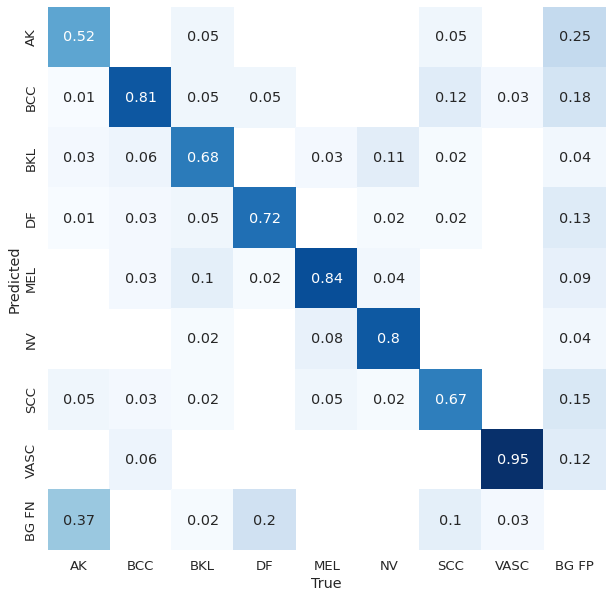
\includegraphics[width=12cm]{img/bab4/confmat-yolov7.png}
        \caption{Hasil \textit{confusion matrix} model terbaik YOLOv7}
        \label{fig:d-confmat-yolov7}
    \end{center}
\end{figure}

Model terbaik YOLOv7 didapatkan dengan 16 nilai \textit{batch size} dan 600 nilai \textit{epochs}. Hasil \textit{confusion matrix} model tersebut seperti terlihat pada Gambar \ref{fig:d-confmat-yolov7}. Seperti terlihat pada Gambar \ref{fig:d-confmat-yolov7}, nilai tertinggi didapatkan oleh kelas VASC. Kanker kulit VASC memiliki ciri khas warna dan bentuk yang signifikan sehingga menjadi kelas yang paling mudah dikenali oleh model YOLOv7. Nilai TP yang rendah didapatkan oleh kelas AK dan SCC. Hal ini juga dapat dipertimbahkan bahwa kanker kulit jenis AK dan SCC memiliki kesamaan dengan area sekitar kulit dan memiliki tepi yang kurang jelas seperti terlihat pada Gambar \ref{fig:ak} dan Gambar \ref{fig:scc}. Hal ini juga dapat dipengaruhi oleh tingkat keparahan jenis kanker yang berbeda-beda. Sedangkan kanker kulit yang berbahaya, yaitu MEL mendapatkan nilai TP sebesar 0.84 yang dapat dikatakan baik untuk klasifikasi. 

\textit{Precision} dan \textit{recall} pada setiap jenis kanker kulit dapat dihitung menggunakan Persamaan \ref{eq:precision} dan \ref{eq:recall}. Perhitungan \textit{precision} dan \textit{recall} seperti terlihat di bawah ini.

\begin{alignat*}{5}
    P_{ak}   &= \frac{TP}{TP+FP}         & R_{ak}   &= \frac{TP}{TP+FP} \\
             &= \frac{0.52}{0.52 + 0.28} &          &= \frac{0.52}{0.52 + 0.4} \\
             &= 0.74                     &          &= 0.75 \\
             &\vdots                     &          &\vdots \\
    P_{vasc} &= \frac{TP}{TP+FP}         & R_{vasc} &= \frac{TP}{TP+FP} \\
             &= \frac{0.95}{0.95 + 0.12} &          &= \frac{0.95}{0.95 + 0.05} \\
             &= 0.97                     &          &= 0.92 \\
\end{alignat*}

Hasil visualisasi \textit{precision} dan \textit{recall} pada model terbaik YOLOv7 seperti terlihat pada Gambar \ref{fig:d-pr-yolov7}.

\begin{figure}[H]
    \begin{center}
        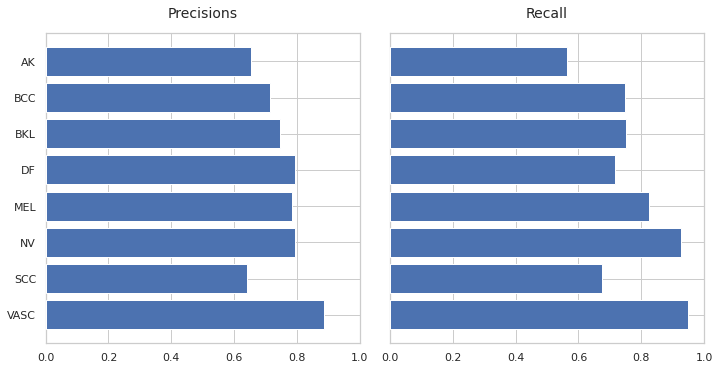
\includegraphics[width=12cm]{img/bab4/pr-yolov7.png}
        \caption{Hasil \textit{precision} dan \textit{recall} model terbaik YOLOv7}
        \label{fig:d-pr-yolov7}
    \end{center}
\end{figure}

Nilai \textit{precision} merepresentasikan tingkat prediksi data negatif sebagai data positif sedangkan nilai \textit{recall} merepresentasikan tingkat prediksi data positif sebagai data negatif. Pada studi kasus diagnosis penyakit, nilai \textit{recall} lebih diutamakan. Hal ini karena \textit{recall} merupakan tingkat sensitifitas model terhadap penyakit tertentu. Pada Gambar \ref{fig:d-pr-yolov7}, terlihat bahwa dari 8 jenis kanker kulit yang diklasifikasikan, nilai \textit{precision} pada semua jenis kanker kulit masih berada di bawah $80\%$ kecuali VASC.  Namun, pada Gambar \ref{fig:d-pr-yolov7} terdapat 3 jenis kanker kulit yang mendekati $80\%$, yaitu DF, MEL, dan NV. Sedangkan nilai \textit{recall} MEL berada di atas $80\%$ beserta jenis kanker NV dan VASC. Nilai \textit{recall} jenis kanker kulit MEL perlu dipertimbangkan karena MEL merupakan jenis kanker kulit paling berbahaya. Nilai \textit{precision} dan \textit{recall} jenis kanker kulit AK dan SCC perlu ditingkatkan lagi dengan menambah \textit{epochs}, data, atau \textit{preprocessing}.

Rendahnya nilai \textit{precision} dan \textit{recall} pada model YOLOv7 dapat dipengaruhi oleh metode YOLOv7 yang tidak dapat melakukan \textit{feature learning} dengan maksimal. Jika YOLOv7 dapat meningkatkan sumber daya pelatihan dengan meningkatkan nilai \textit{epochs} maka tidak menutup kemungkinan bahwa nilai \textit{precision} dan \textit{recall} dapat meningkat. Hal tersebut juga dapat dipengaruhi oleh kurangnya jumlah data pada dataset karena pengembang YOLO mengatakan bahwa jumlah minimal data citra untuk satu kelas adalah 1500 data \citep{Jocher2020}. Sedangkan, penelitian ini hanya menggunakan 200 data pada tiap kelas di dataset. 

\begin{figure}[H]
    \begin{center}
        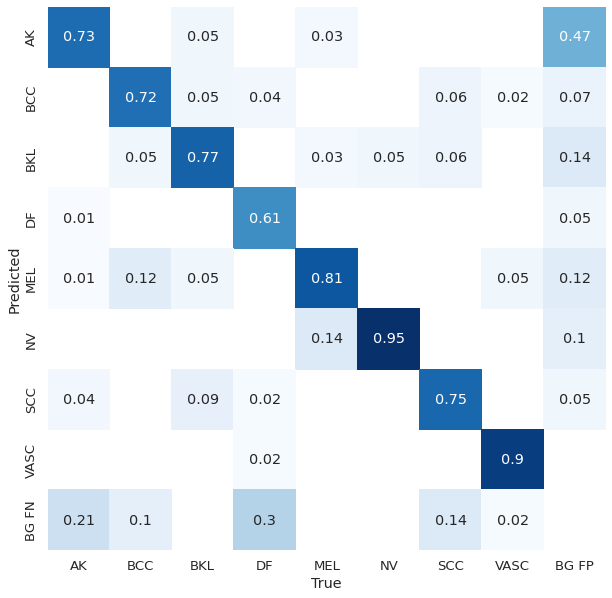
\includegraphics[width=12cm]{img/bab4/confmat-yolov7tiny.png}
        \caption{Hasil \textit{confusion matrix} model terbaik YOLOv7 Tiny}
        \label{fig:d-confmat-yolov7tiny}
    \end{center}
\end{figure}

Hasi visualisasi \textit{confusion matrix} model YOLOv7 Tiny terbaik seperti terlihat pada Gambar \ref{fig:d-confmat-yolov7tiny}. Nilai TP tertinggi yang dihasilkan dari model YOLOv7 Tiny sebesar $95\%$ oleh jenis kanker kulit NV. Pada model YOLOv7 Tiny, kanker kulit jenis AK dan SCC lebih mudah dikenali daripada kanker kulit DF. Bahkan, kanker kulit jenis AK memiliki nilai TP sebesar $73\%$ pada YOLOv7 Tiny sedangkan kanker kulit jenis DF memiliki nilai TP sebesar $61\%$. Ketiga jenis kanker kulit yang memiliki nilai TP tertinggi adalah MEL, NV, dan VASC. Keberhasilan model dalam mendeteksi jenis kanker kulit dapat dilihat dari nilai \textit{precision} dan \textit{recall} seperti perhitungan di bawah ini.

\begin{alignat*}{5}
    P_{ak}   &= \frac{TP}{TP+FP}         & R_{ak}   &= \frac{TP}{TP+FP} \\
             &= \frac{0.73}{0.73 + 0.26} &          &= \frac{0.73}{0.73 + 0.24} \\
             &= 0.74                     &          &= 0.75 \\
             &\vdots                     &          &\vdots \\
    P_{vasc} &= \frac{TP}{TP+FP}         & R_{vasc} &= \frac{TP}{TP+FP} \\
             &= \frac{0.90}{0.90 + 0.02} &          &= \frac{0.90}{0.90 + 0.08} \\
             &= 0.97                     &          &= 0.92 \\
\end{alignat*}

Hasil visualisasi perhitungan \textit{precision} dan \textit{recall} pada perhitungan di atas dapat dilihat pada Gambar \ref{fig:d-pr-yolov7tiny}.

\begin{figure}[H]
    \begin{center}
        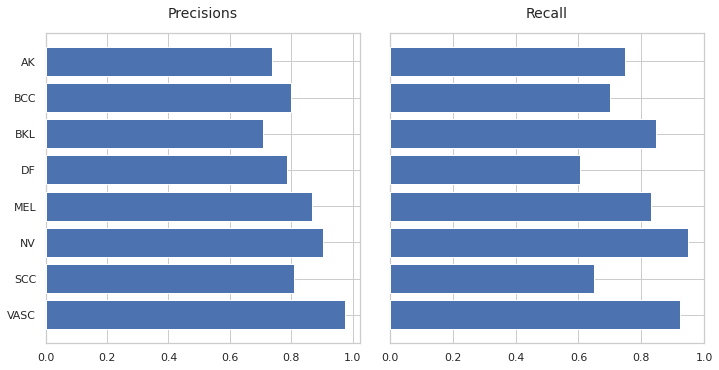
\includegraphics[width=12cm]{img/bab4/pr-yolov7tiny.png}
        \caption{Hasil \textit{precision} dan \textit{recall} model terbaik YOLOv7 Tiny}
        \label{fig:d-pr-yolov7tiny}
    \end{center}
\end{figure}

Gambar \ref{fig:d-pr-yolov7tiny} menunjukkan bahwa model dapat mengenali jenis kanker kulit jenis MEL, NV, dan VASC dengan baik. Pada studi kasus klasifikasi penyakit, nilai \textit{recall} sangat diperhitungkan untuk mengetahui tingkat sensitifitas model terhadap penyakit dengan tidak melupakan nilai \textit{precision}. Pada Gambar \ref{fig:d-pr-yolov7tiny}, nilai \textit{recall} yang tinggi didapatkan oleh kanker kulit jenis NV dan VASC.

Berdasarkan nilai \textit{precision} dan \textit{recall} dapat dihitung nilai mAP menggunakan Persamaan \ref{eq:map}. Contoh perhitungan mAP seperti perhitungan di bawah ini.

\begin{alignat*}{5}
    AP_{ak}     &= &&\sum_{i=0}^{n-1} \left( (R_i - R_{i+1})\times P_i \right) \\
                &= &&\left( (0.97-0.95)\times 0.21 \right) + \left( (0.95-0.91)\times 0.32 \right) + \\
                &  &&\left( (0.91-0.87)\times 0.32 \right) + \cdots + \left( (0.12 - 0.02)\times 0.98 \right) \\
                &= &&0.527 \\
                &  &&\vdots \\
    AP_{vasc}   &= &&\sum_{i=0}^{n-1} \left( (R_i - R_{i+1})\times P_i \right) \\
                &= &&\left( (0.99-0.98)\times 0.25 \right) + \left( (0.98-0.95)\times 0.27 \right) + \\
                &  &&\left( (0.95-0.92)\times 0.41 \right) + \cdots + \left( (0.21 - 0.19)\times 0.96 \right) \\
                &= &&0.93
\end{alignat*}

Hasil visualisasi perhitungan di atas seperti terlihat pada Gambar \ref{fig:d-map}.

\begin{figure}[H]
    \begin{center}
        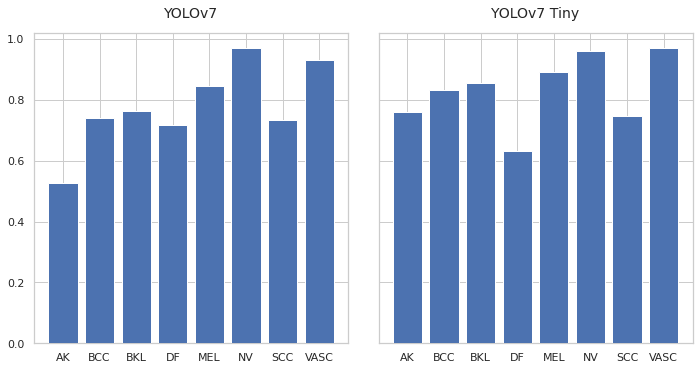
\includegraphics[width=12cm]{img/bab4/map.png}
        \caption{Hasil mAP model terbaik YOLOv7 dan YOLOv7 Tiny}
        \label{fig:d-map}
    \end{center}
\end{figure}

Pada Gambar \ref{fig:d-map}, nilai mAP yang tinggi didapatkan oleh jenis kanker kulit NV dan VASC pada YOLOv7 maupun YOLOv7 Tiny. Nilai mAP pada jenis kanker paling berbahaya, yaitu MEL juga cukup signifikan. Pada YOLOv7, nilai mAP yang perlu ditingkatkan adalah jenis kanker kulit AK. Akan tetapi, jenis kanker kulit AK memiliki nilai yang tidak terlalu buruk pada model YOLOv7 Tiny. Hal ini dapat dipengaruhi oleh arsitektur model. Pada YOLOv7 Tiny tidak menggunakan ELAN dan fungsi aktivasi SiLU, akan tetapi komposisi \textit{convolutional layer} dengan beberapa \textit{skip connections} dan \textit{concatenation}. Hal ini justru membuat YOLOv7 Tiny dapat mempelajari pola data dari jenis kanker kulit AK. Fungsi aktivasi Leaky ReLU pada YOLOv7 Tiny juga dapat berpengaruh karena fungsi aktivasi SiLU hanya meneruskan nilai yang lebih dari 0. Berbeda dengan fungsi aktivasi SiLU pada YOLOv7 dengan perhitungan yang lebih kompleks seperti terlihat pada Persamaan \ref{eq:silu}. 

Pada model YOLOv7 Tiny, jenis kanker kulit dengan nilai mAP terendah didapatkan oleh jenis kanker kulit DF. Sebaliknya, jenis kanker kulit DF memiliki nilai mAP yang tidak terlalu buruk pada model YOLOv7. Dapat dilihat pada Gambar \ref{fig:d-map} bahwa rata-rata jenis kanker kulit memiliki nilai mAP lebih tinggi pada model YOLOv7 Tiny daripada model YOLOv7. Keunggulan YOLOv7 Tiny juga memiliki waktu komputasi yang lebih cepat. Hal ini disebabkan oleh kompleksitas arsitektur yang ada pada YOLOv7 Tiny lebih rendah daripada kompleksitas arsitektur yang ada pada YOLOv7 dengan mempertimbangkan ELAN dan fungsi aktivasi SiLU. Fungsi aktivas Leaky ReLU cukup baik meningkatkan kinerja model YOLOv7 Tiny. Pada penelitian ini dengan dataset kanker kulit yang terdiri dari 8 kelas, model YOLOv7 Tiny cukup memberikan nilai mAP yang tinggi dengan waktu komputasi yang lebih cepat. Pembaruan yang dibawa oleh Wang, dkk. terkait ELAN dan fungsi aktivasi SiLU belum dapat dirasakan pada penelitian ini.

\section{Integrasi Keilmuan}

Hasil penelitian ini memberikan pengingat yang luar biasa terkait perkembangan zaman. Semakin jauh perkembangan zaman, semakin kompleks permasalahan yang dihadapi. Hal ini linier dengan perkembangan solusi untuk menyelesaikan masalah yang terjadi. Salah satunya adalah perkembangan metode untuk melakukan diagnosis kanker kulit. Selain dari rahmat Allah \textit{subhanallahu wa ta'ala}, hal ini tercapai atas kemauan manusia berusaha dalam menghadapi permasalahan yang ada sebagaimana firman-Nya dalam surat Ar-Ra'd ayat 11:

\begin{flushright}
    \begin{RLtext}
        لَهُۥ مُعَقِّبَٰتٌ مِّنۢ بَيْنِ يَدَيْهِ وَمِنْ خَلْفِهِۦ يَحْفَظُونَهُۥ مِنْ أَمْرِ ٱللَّهِ ۗ إِنَّ ٱللَّهَ لَا يُغَيِّرُ مَا بِقَوْمٍ حَتَّىٰ يُغَيِّرُوا۟ مَا بِأَنفُسِهِمْ ۗ وَإِذَآ أَرَادَ ٱللَّهُ بِقَوْمٍ سُوٓءًا فَلَا مَرَدَّ لَهُۥ ۚ وَمَا لَهُم مِّن دُونِهِۦ مِن وَالٍ
    \end{RLtext}
\end{flushright}

Artinya: "Bagi manusia ada malaikat-malaikat yang selalu mengikutinya bergiliran, di muka dan di belakangnya, mereka menjaganya atas perintah Allah. Sesungguhnya Allah tidak merubah keadaan sesuatu kaum sehingga mereka merubah keadaan yang ada pada diri mereka sendiri. Dan apabila Allah menghendaki keburukan terhadap sesuatu kaum, maka tak ada yang dapat menolaknya; dan sekali-kali tak ada pelindung bagi mereka selain Dia." (Ar-Ra'd: 11).

Ayat tersebut menjelaskan bahwa kesungguhan manusia akan membuahkan hasil. Semua usaha manusia tidak akan ada yang sia-sia sehingga Allah \textit{subhanallahu wa ta'ala} tidak memberikan balasan yang sesuai. Bahkan, Allah \textit{subhanallahu wa ta'ala} tidak akan mengubah keadaan suatu kaum hingga mereka mengubah keadaan yang ada pada diri mereka sendiri. Jika saja manusia tidak berusaha untuk menemukan solusi terkait permasalahan, seperti contoh pada penelitian ini adalah penyakit kanker kulit pasti Allah \textit{subhanallahu wa ta'ala} tidak akan memberikan jalan untuk menemukan metode-metode yang dapat menyelesaikan proses klasifikasi kanker kulit dengan hasil yang cukup baik.

Hasil pada penelitian ini menggambarkan kerja keras umat manusia dalam berlomba-lomba dalam bidang keilmuan. Namun, hal itu tidak akan tercapai jika tidak dengan rahmat Allah \textit{subhanallahu wa ta'ala}. Hal tersebut juga salah satu dari bentuk ikhtiar seorang hamba kepada Allah \textit{subhanallahu wa ta'ala}. Allah \textit{subhanallahu wa ta'ala} yang memilki kuasa atas kesembuhan terkait penyakit yang menimpa sebagaimana firman-Nya dalam surat Asy-Syu'ara ayat 80:

\begin{flushright}
    \<وَإِذَا مَرِضْتُ فَهُوَ يَشْفِينِ>
\end{flushright}

Artinya: "Dan apabila aku sakit, Dialah Yang menyembuhkan aku," (QS: Asy-Syu'ara: 80, Al-Anbiyaa': 83).

Berdasarkan ayat di atas, Allah \textit{subhanallahu wa ta'ala} yang melimpahkan umat manusia kenikmatan makanan dan minuman. Jika suatu penyakit menimpa umat manusia, maka Allah \textit{subhanallahu wa ta'ala} yang akan menyembuhkannya. Hal ini sejalan dengan firman-Nya dalam surah Al-Anbiyaa' ayat 83:

\begin{flushright}
    \<وَأَيُّوبَ إِذْ نَادَىٰ رَبَّهُۥٓ أَنِّى مَسَّنِىَ ٱلضُّرُّ وَأَنتَ أَرْحَمُ ٱلرَّٰحِمِينَ>
\end{flushright}

Kedua ayat di atas memaparkan bahwa ketika suatu penyakit menimpa umat manusia, hanya Allah \textit{subhanallahu wa ta'ala} yang dapat menyembuhkannya. Hal tersebut dapat diteladani dari kisah Nabi Ibrahim \textit{'alaihissalam} dan Nabi Ayyub \textit{'alaihissalam} sebagaimana kedua ayat di atas. Ketika Allah \textit{subhanallahu wa ta'ala} memberikan kesembuhan, manusia wajib untuk bersyukur kepada-Nya sebagaimana firman-Nya dalam surat Al-Baqarah ayat 152:

\begin{flushright}
    \<فَٱذْكُرُونِىٓ أَذْكُرْكُمْ وَٱشْكُرُوا۟ لِى وَلَا تَكْفُرُونِ>
\end{flushright}

Pada ayat di atas, Allah \textit{subhanallahu wa ta'ala} memerintahkan manusia untuk mengingat-Nya, bersyukur kepada-Nya, dan tidak kufur kepada-Nya. Sebagaimana dengan hasil pada penelitian ini, harus diingat bahwa hasil tersebut tidak akan tercapai jika tidak sesuai dengan kehendak Allah \textit{azza wa jalla}. Maka dari itu, jangan kufur terhadap nikmat-nikmat Allah \textit{subhanallahu wa ta'ala} dengan mengingkari nikmat-nikmat-Nya dan menggunakannya untuk perkara yang diharamkan oleh Allah \textit{subhanallahu wa ta'ala}.

